\documentclass[xcolor=pdftex,dvipsnames,table,mathserif]{beamer}
%\usepackage{subfigure}
\usepackage{amsbsy}
\usepackage{tikz}
\usetikzlibrary{arrows}
\usepackage{amsmath,graphicx,dsfont,color}
\usepackage{amsfonts}
\usepackage{amssymb}
\usepackage{array}

\usepackage{subfig}

% makes the subfig package work
\makeatletter
\let\@@magyar@captionfix\relax
\makeatother

% subfigure counter resets every frame
\makeatletter
\@addtoreset{subfigure}{framenumber}
\makeatother

% First author and year
\bibliographystyle{apalike}

% This sets the list items of the bibliography to the same symbol used for citation.
\setbeamertemplate{bibliography item}{\insertbiblabel}

% This avoids extralines for different entries
\setbeamertemplate{bibliography entry title}{}
\setbeamertemplate{bibliography entry location}{}
\setbeamertemplate{bibliography entry note}{}

\DeclareMathOperator*{\argmin}{arg\,min}
\DeclareMathOperator*{\argmax}{arg\,max}
%Definitiona

\newcommand{\x}{\mathbf{x}}
\newcommand{\X}{\mathbf{X}}
\newcommand{\W}{\mathbf{W}} %Weight
\newcommand{\bais}{\mathbf{b}}%Bais
\newcommand{\act}{\texttt{g}}%Activation
\newcommand{\loss}{L}
\newcommand{\pdata}{\hat{p}_{\texttt{data}}}
\newcommand{\nsize}{N}
\newcommand{\nfeatures}{P}
\newcommand{\param}{\boldsymbol{\theta}}
\newcommand{\featmap}{\boldsymbol{\phi}}
\newcommand{\EV}{\mathbb{E}}







\usepackage{physics}

\graphicspath{{../graphics/}}

\AtBeginSection[]{
  \begin{frame}{Contents}
    \tableofcontents[currentsection, hideothersubsections]
  \end{frame}
}

\AtBeginSubsection[]{
  \begin{frame}{Contents}
    \tableofcontents[currentsection, subsectionstyle=show/shaded/hide]
  \end{frame}
}

\setbeamertemplate{footline}[frame number]{}
\setbeamertemplate{navigation symbols}{}
\setbeamertemplate{section in toc}[square]
\setbeamertemplate{items}[square]

%% For image credits on image bottom right
\usepackage[absolute,overlay]{textpos}
\setbeamercolor{framesource}{fg=gray}
\setbeamerfont{framesource}{size=\tiny}
\newcommand{\source}[1]{\begin{textblock*}{4cm}(8.7cm,8.6cm)
    \begin{beamercolorbox}[ht=0.5cm,right]{framesource}
      \usebeamerfont{framesource}\usebeamercolor[fg]{framesource} Credits: {#1}
    \end{beamercolorbox}
\end{textblock*}}

\title{Unsupervised anomalous image detection}
\author{E. Decencière}
\date{MINES ParisTech\\
  PSL Research University\\
  Center for Mathematical Morphology
}
\titlegraphic{
\includegraphics[height=1.7cm]{../graphics/logoemp}}

\useinnertheme{rounded}
\usecolortheme{rose}

%%%%%%%%%%%%%%%%%%%%%%%%%%%%%%%%%%%%%%%%%%%%%%%%%%%%%%%
%%%%%%%%%%%%%%%%%%%%%%%%%%%%%%%%%%%%%%%%%%%%%%%%%%%%%%%

\begin{document}

\frame{\titlepage}

\frame{
  \frametitle{Contents}
  \tableofcontents[hidesubsections]
}

%%%%%%%%%%%%%%%%%%%%%%%%%%%%%%%%%%%%%%%%%%%%%%%%%%
%%%%%%%%%%%%%%%%%%%%%%%%%%%%%%%%%%%%%%%%%%%%%%%%%%
\section{Introduction}

%%%%%%%%%%%%%%%%%%%%%%%%%%%%%%%%%%%%
\begin{frame}{Diabetic retinopathy screening}

  \begin{columns}
    \begin{column}{.5\textwidth}
  \begin{figure}[ht]
    \centering
    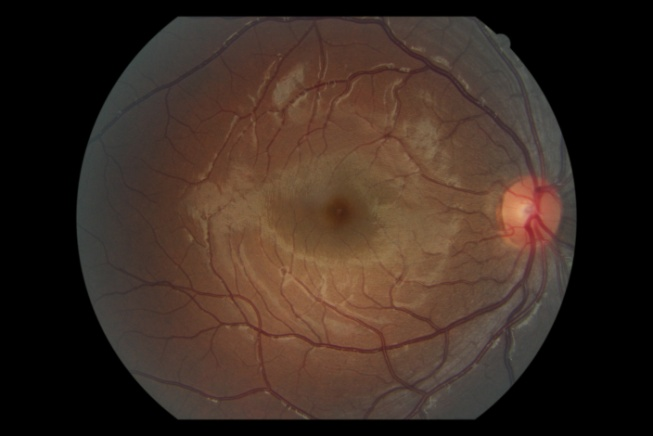
\includegraphics[width=\textwidth]{fundus1}
    \caption*{Normal image}
  \end{figure}

    \end{column}

    \begin{column}{.5\textwidth}

\begin{figure}[ht]
  \centering
  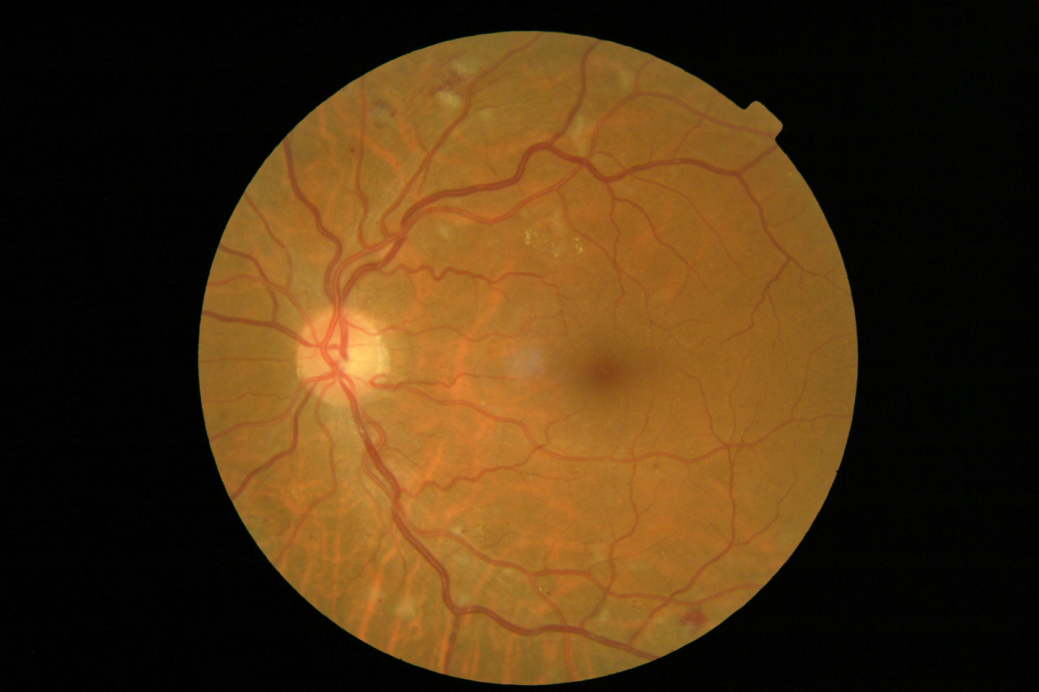
\includegraphics[width=\textwidth]{ret-dr}
  \caption*{Fundus with signs of diabetic retinopathy}
\end{figure}


    \end{column}
  \end{columns}

      \source{OPHDIAT database}

\end{frame}


%%%%%%%%%%%%%%%%%%%%%%%%%%%%%%%%%%%%
\begin{frame}{Specific methods}

\begin{columns}
  \begin{column}{.5\textwidth}
    \begin{figure}[ht]
      \centering
      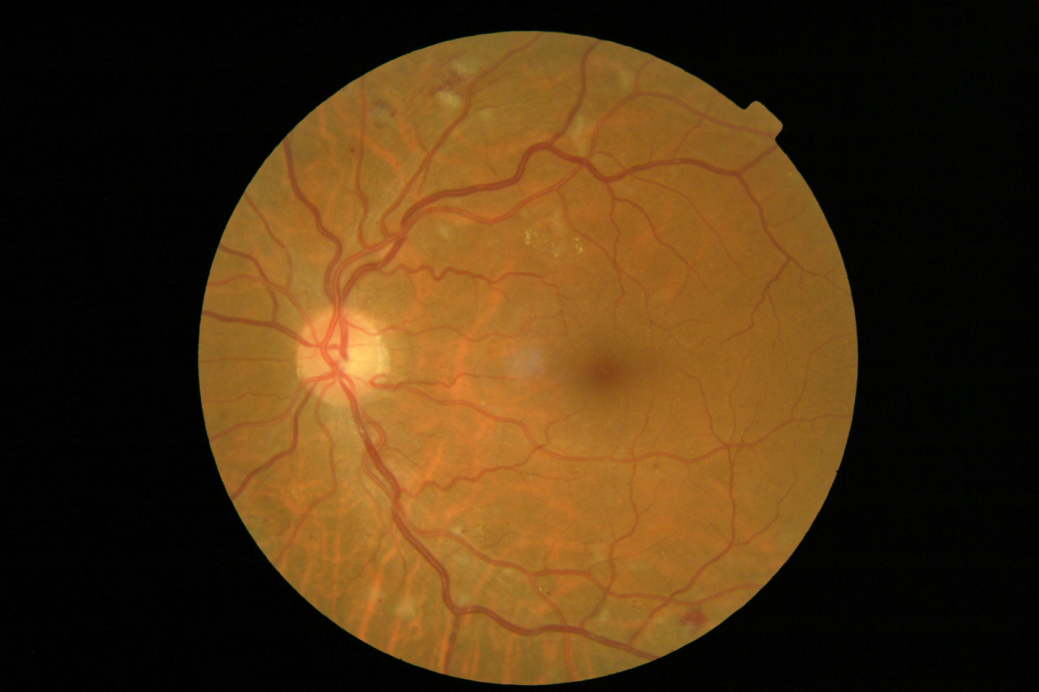
\includegraphics[width=\textwidth]{ret-dr}
      \caption*{Original image}
    \end{figure}

  \end{column}

  \begin{column}{.5\textwidth}
\begin{figure}[ht]
  \centering
  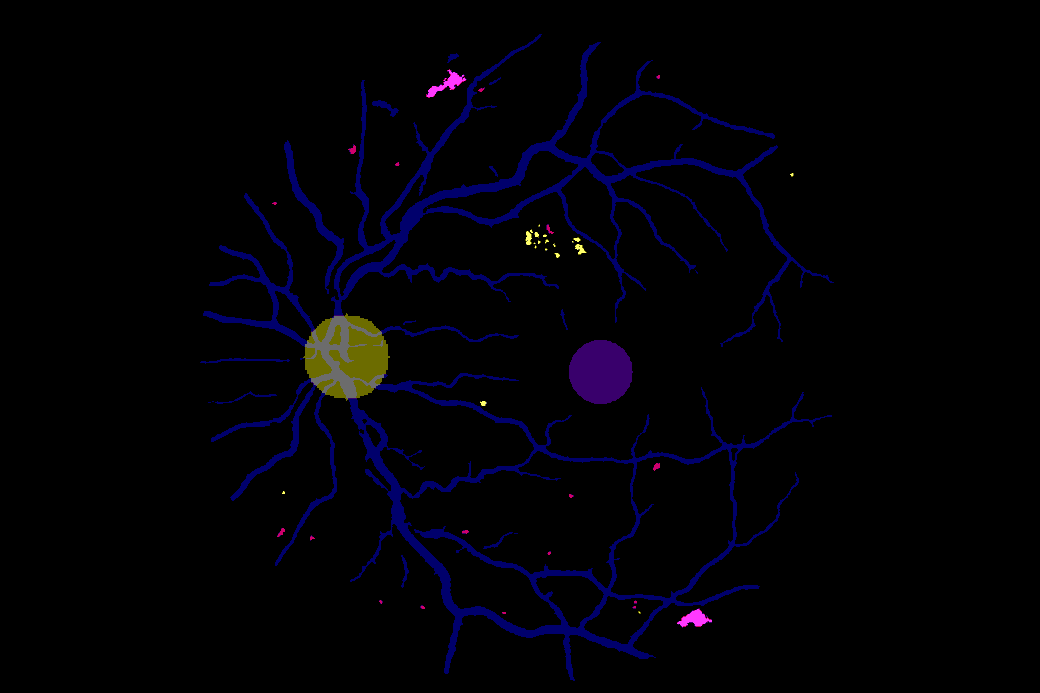
\includegraphics[width=\textwidth]{ret-dr-segm}
  \caption*{Segmentation of anatomical and pathological structures}
\end{figure}

  \end{column}
\end{columns}

\end{frame}


%%%%%%%%%%%%%%%%%%%%%%%%%%%%%%%%%%%%
\begin{frame}{Unexpected case}

\begin{figure}[ht]
  \centering
  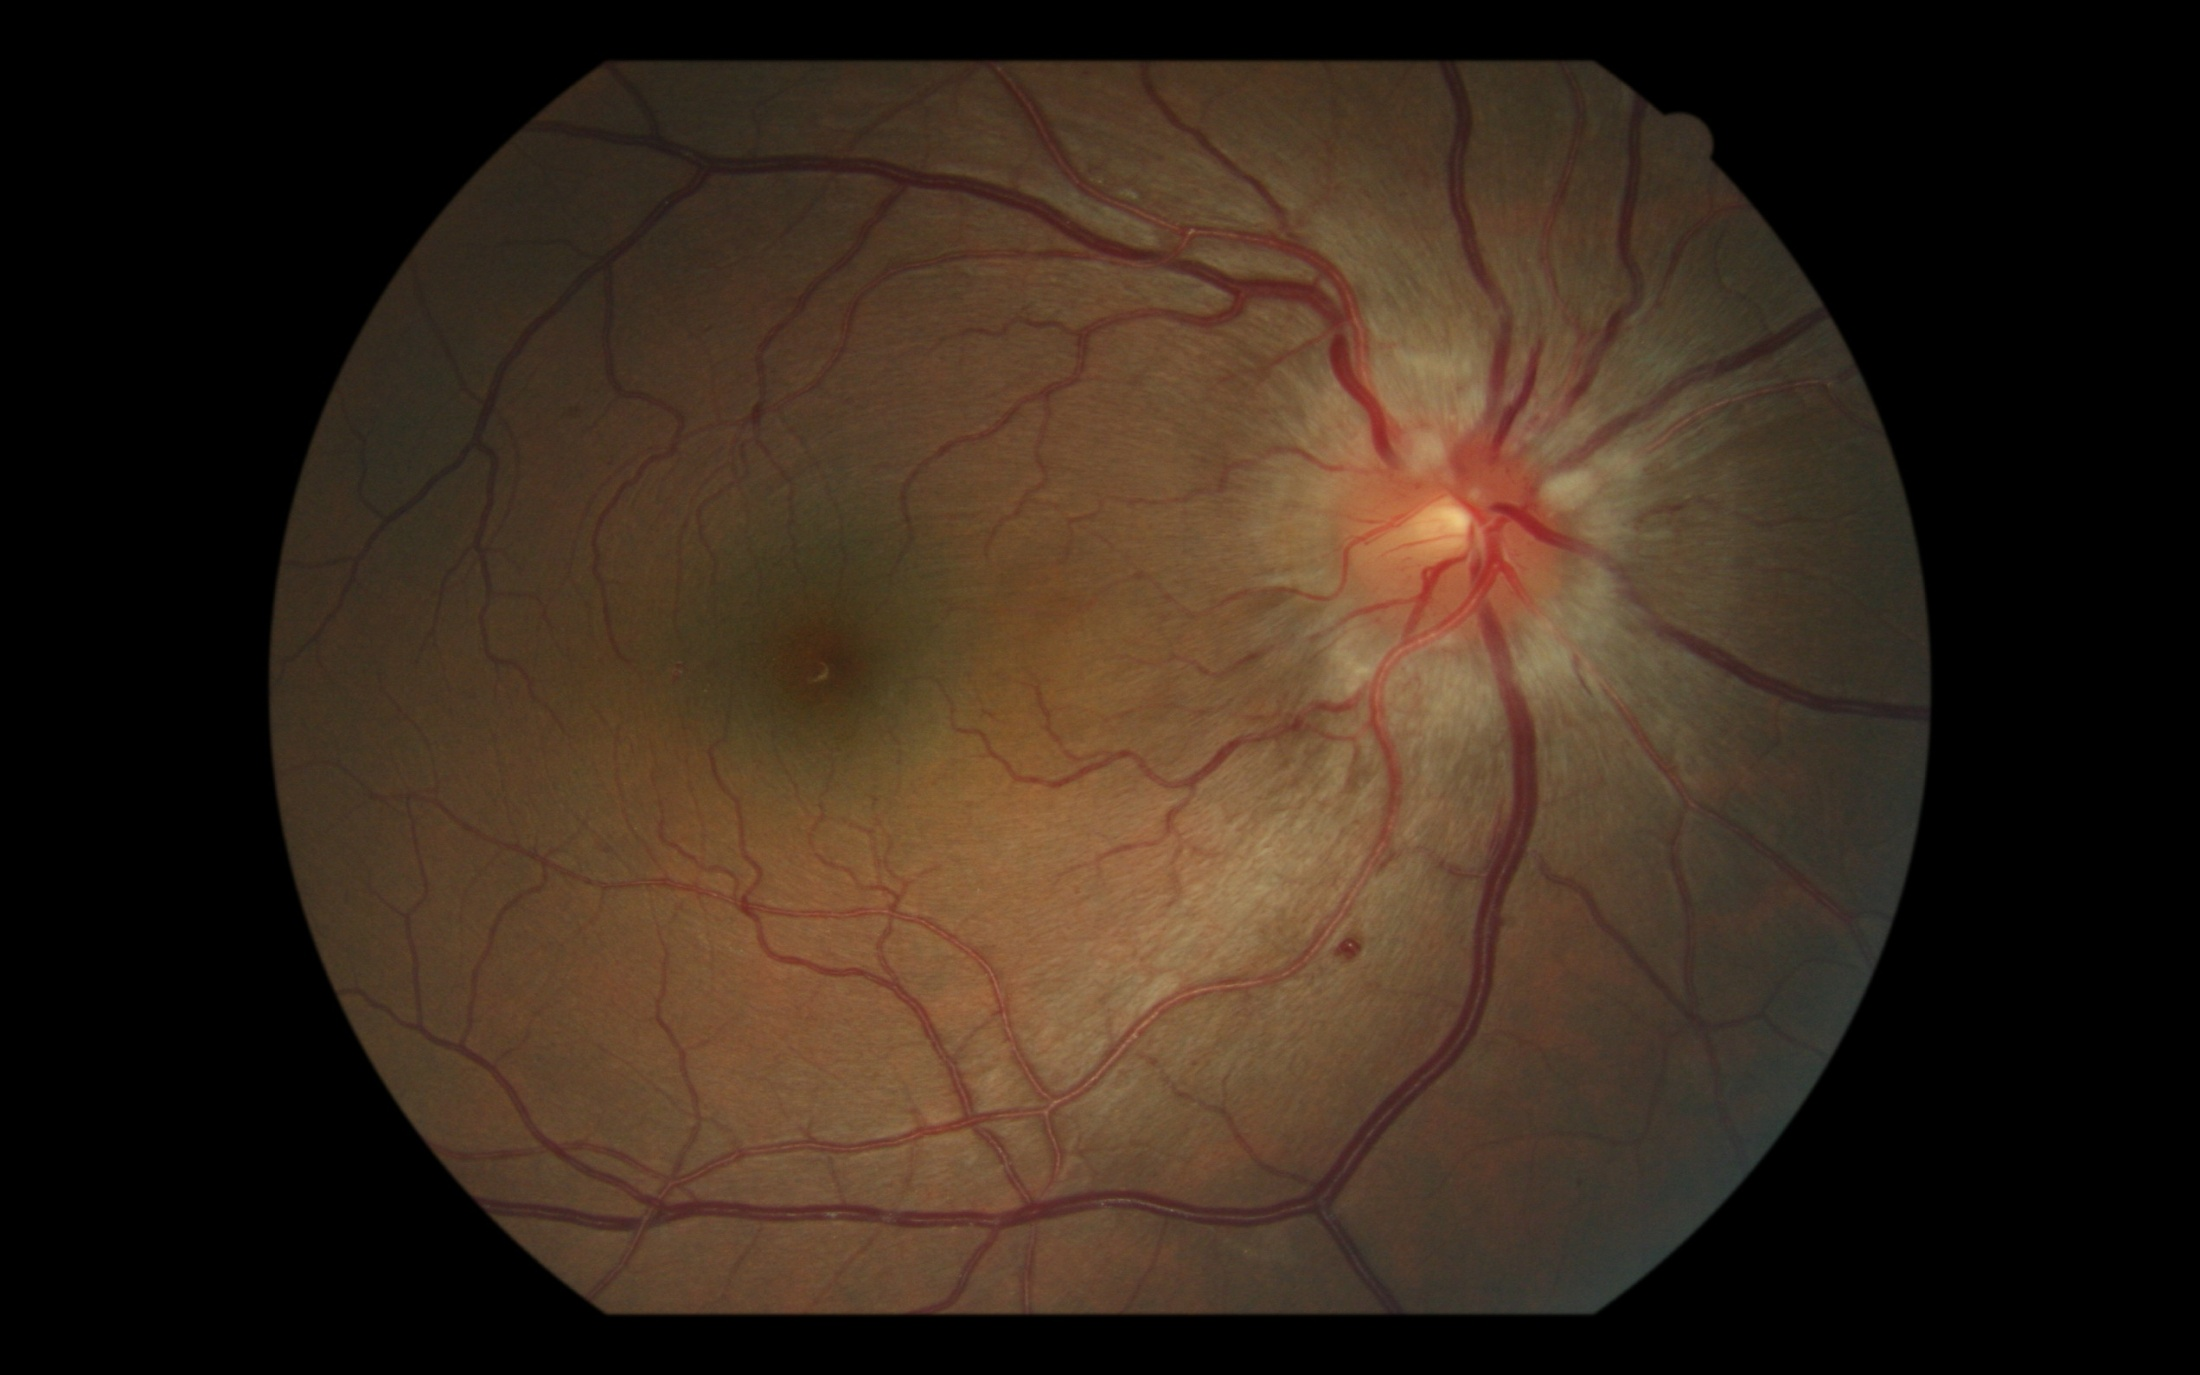
\includegraphics[width=0.5\textwidth]{ret-oedeme}
  \caption*{Papilledema}
\end{figure}


\end{frame}


%%%%%%%%%%%%%%%%%%%%%%%%%%%%%%%%%%%%
\begin{frame}{Definition in layman terms}

  \begin{block}{Classical definition \cite{hawkins_identification_1980}}
    ``An observation which deviates so much from other observations as to arouse suspicions that it was generated by a different mechanism''.
  \end{block}

\end{frame}

%%%%%%%%%%%%%%%%%%%%%%%%%%%%%%%%%%%%
\begin{frame}{Definition in layman terms}

  \begin{block}{Anomalous image detection in a learning framework}
    \begin{itemize}
    \item Let us consider a given set of images. Among these, some  are defined as being \alert{normal}. The aim of the detection task is to decide, for any given image, if it is normal, or not.
    \item The definition of normal images is given through a set of examples.
    \end{itemize}
  \end{block}

  \begin{itemize}
  \item We will focus on images, but the problem is very general.
  \item We will suppose that we only have examples of normal images, i.e.\ that we are in a \alert{unsupervised} context. We assume that examples of anomalies are not representative enough or unknown.
  \end{itemize}



\end{frame}

%%%%%%%%%%%%%%%%%%%%%%%%%%%%%%%%%%%%
\begin{frame}{Example - set of normal images}

  \begin{figure}[ht]
    \centering
    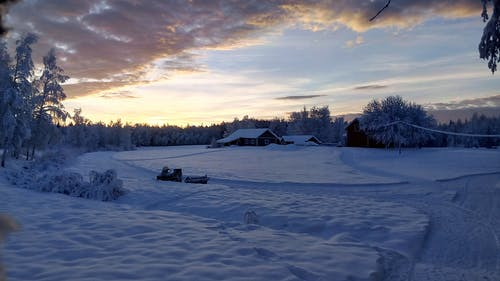
\includegraphics[width=0.3\textwidth]{snow1-pexels-photo-290548.jpg}
    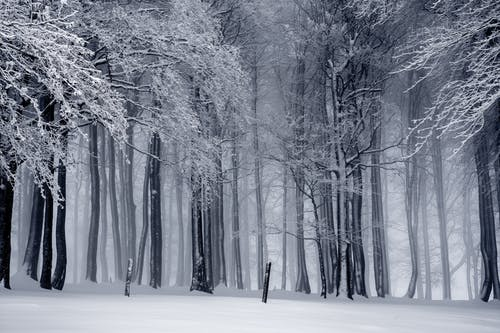
\includegraphics[width=0.3\textwidth]{snow2-pexels-photo-235621.jpg}
    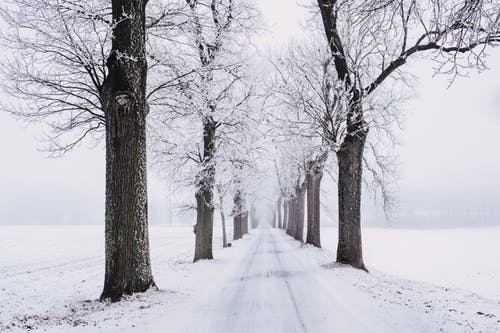
\includegraphics[width=0.3\textwidth]{snow3-pexels-photo-839462.jpeg}
    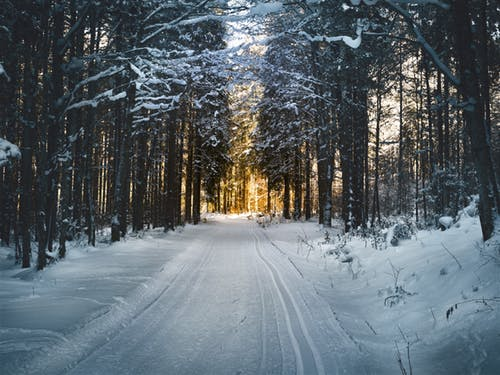
\includegraphics[width=0.3\textwidth]{snow4-pexels-photo-688660.jpeg}
    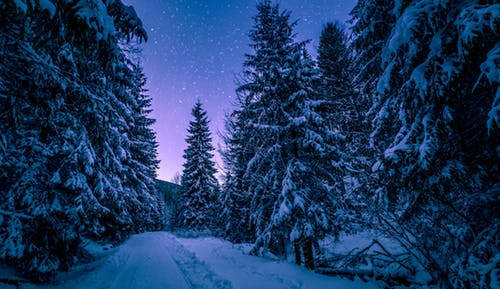
\includegraphics[width=0.3\textwidth]{snow5-pexels-photo-773594.jpeg}
    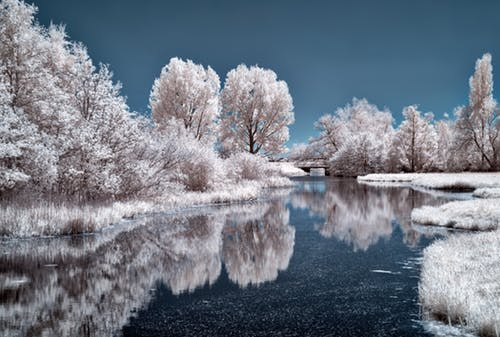
\includegraphics[width=0.3\textwidth]{snow6-pexels-photo-1559117.jpeg}
    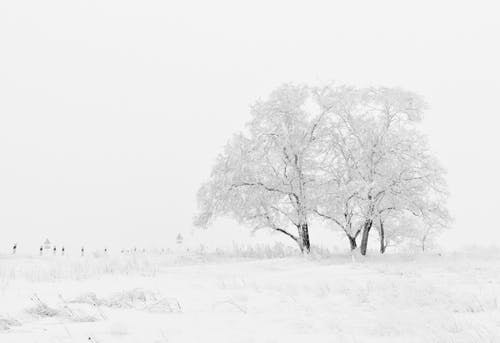
\includegraphics[width=0.3\textwidth]{snow7-pexels-photo-66284.jpeg}
    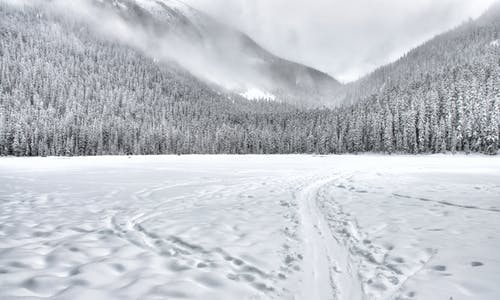
\includegraphics[width=0.3\textwidth]{snow8-pexels-photo-1571442.jpeg}
    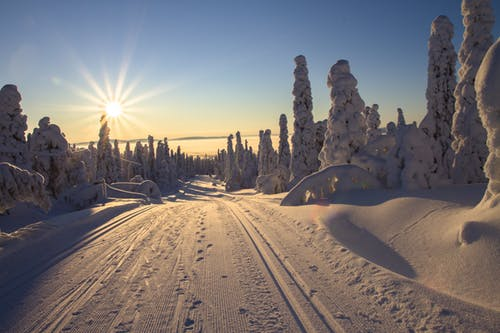
\includegraphics[width=0.3\textwidth]{snow9-pexels-photo-416728.jpeg}\
    \source{http://pexels.com}
  \end{figure}

\end{frame}

%%%%%%%%%%%%%%%%%%%%%%%%%%%%%%%%%%%%
\begin{frame}{Example - which images are normal?}

  \begin{figure}[ht]
    \centering
    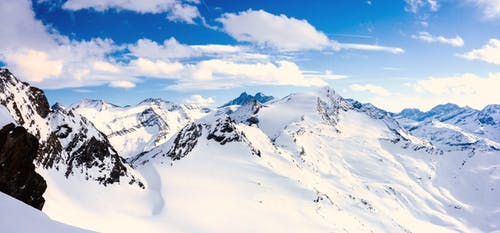
\includegraphics[width=0.3\textwidth]{test1-pexels-photo-414459.jpeg}
    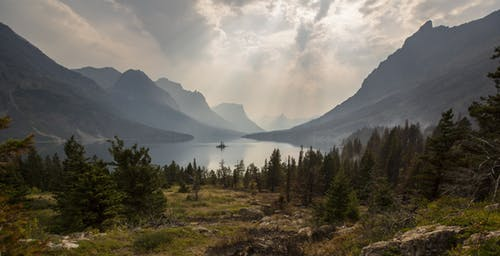
\includegraphics[width=0.3\textwidth]{test2-pexels-photo-414171.jpeg}
    \source{http://pexels.com}
  \end{figure}

\end{frame}


%%%%%%%%%%%%%%%%%%%%%%%%%%%%%%%%%%%%
\begin{frame}{Medicine}

  \begin{itemize}
  \item Detection of suspicious conditions
  \item Non specific screening
  \end{itemize}

\begin{block}{Rare conditions}
  For medical diagnostic or screening applications, it is extremely difficult to have a complete list of possible pathologies - and in any cases the number of examples of rare conditions will always be small.
\end{block}



\end{frame}



%%%%%%%%%%%%%%%%%%%%%%%%%%%%%%%%%%%%
\begin{frame}{Application: security}


  \begin{block}{Suspicious object or unusual behaviour in a scene}
    \begin{figure}[ht]
      \centering
      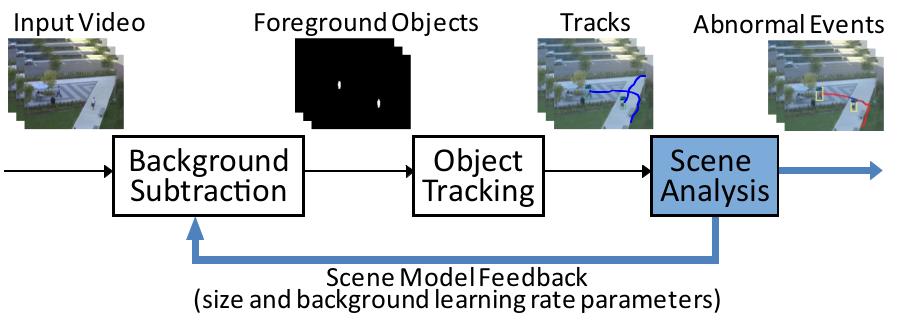
\includegraphics[width=\textwidth]{motion_patterns_anom_det}
      \source{\cite{basharat_learning_2008}}
    \end{figure}

  \end{block}

\end{frame}

%%%%%%%%%%%%%%%%%%%%%%%%%%%%%%%%%%%%
\begin{frame}{Application: security}

  \begin{block}{Examples of normal images}
    \begin{figure}[ht]
      \centering
      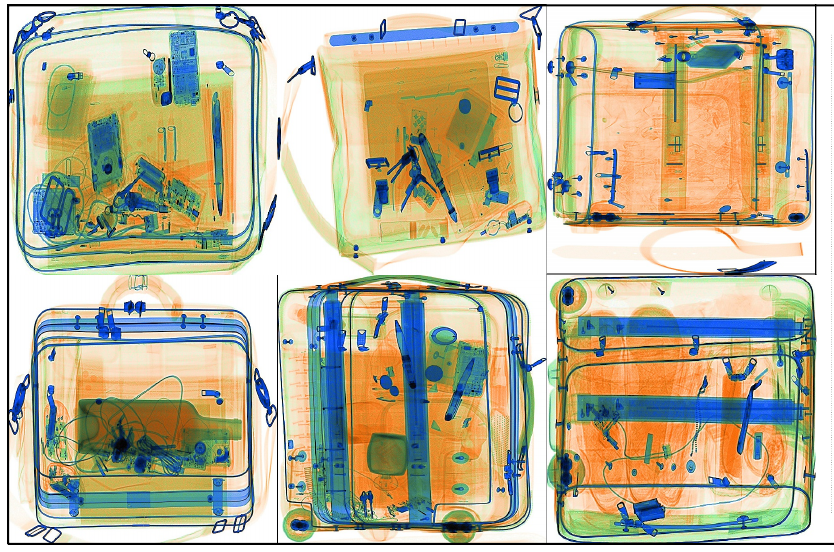
\includegraphics[height=0.5\textheight]{xray-secu-train}
      \source{\cite{akcay_ganomaly:_2019}}
    \end{figure}
  \end{block}

\end{frame}


%%%%%%%%%%%%%%%%%%%%%%%%%%%%%%%%%%%%
\begin{frame}{Application: security (cont.)}

  \begin{block}{Examples of test images}
    \begin{figure}[ht]
      \centering
      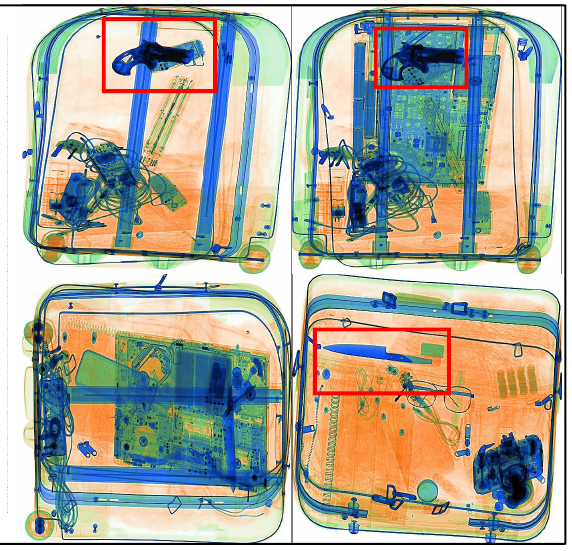
\includegraphics[height=0.5\textheight]{xray-secu-test}
      \source{\cite{akcay_ganomaly:_2019}}
    \end{figure}

  \end{block}

\end{frame}



%%%%%%%%%%%%%%%%%%%%%%%%%%%%%%%%%%%%
\begin{frame}{Application: industrial control}

  \begin{itemize}
  \item Fault detection
  \item Structural defect detection
  \end{itemize}

  \begin{figure}[ht]
    \centering
    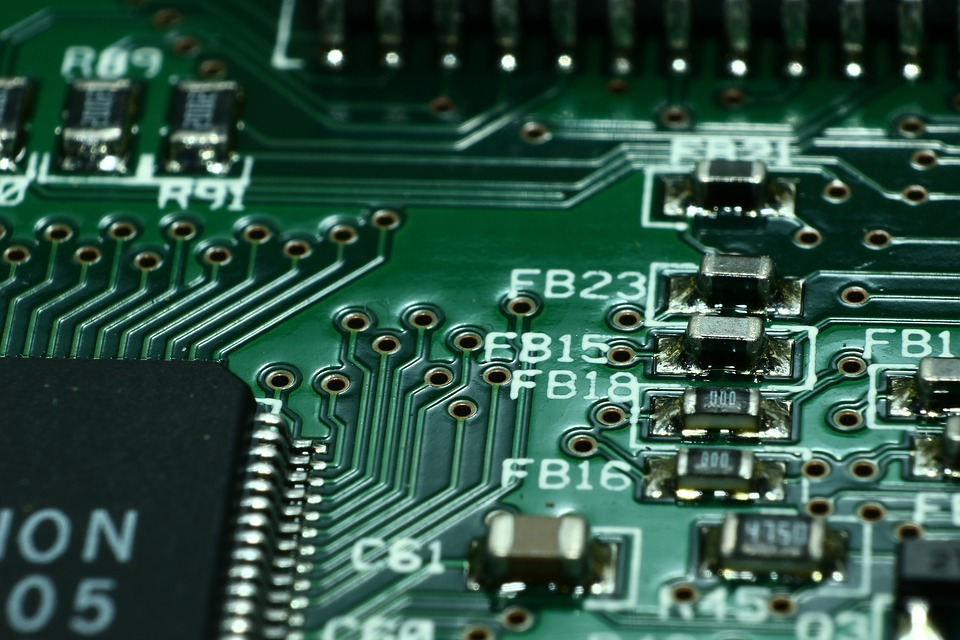
\includegraphics[width=0.5\textwidth]{printed-circuit-board-1539113_960_720.jpg}
    \source{http://www.pixabay.com}
  \end{figure}


\end{frame}

%%%%%%%%%%%%%%%%%%%%%%%%%%%%%%%%%%%%
\begin{frame}{Science}

\begin{block}{}
The most exciting phrase to hear in science, the one that heralds new discoveries, is not “Eureka!” (I found it!) but “That’s funny \ldots”

— Isaac Asimov

\end{block}

Discrepancy between an observation and a model motivates new research.

\end{frame}


%%%%%%%%%%%%%%%%%%%%%%%%%%%%%%%%%%%%
\begin{frame}{Science}

  \begin{itemize}
  \item In some fields so many images are generated that it is becoming impossible to look at all of them
  \item Example: Euclid telescope (European Space Agency and Euclid consortium)
  \end{itemize}

  \begin{figure}[ht]
    \centering
    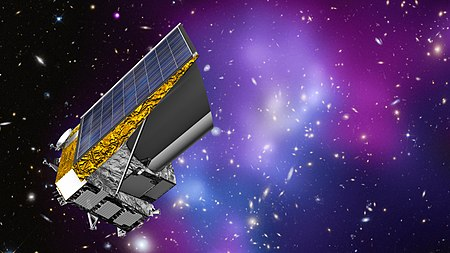
\includegraphics[width=0.5\textwidth]{450px-Euclid_ESA376594}
    \source{https://sci.esa.int/web/euclid/}
  \end{figure}


\end{frame}


%%%%%%%%%%%%%%%%%%%%%%%%%%%%%%%%%%%%
\begin{frame}{Euclid project}

  \begin{itemize}
  \item A new space telescope, to be launched in 2022
  \item Its objective is improving our understanding of the acceleration of the universe expansion
  \item To do so, the shapes of galaxies at different distances from the earth will be measured
  \item An estimated $10^{10}$ extra galactic objects will be acquired by the telescope
  \item Data will be automatically analyzed, without visual inspection
  \end{itemize}

  \begin{figure}[ht]
    \centering
    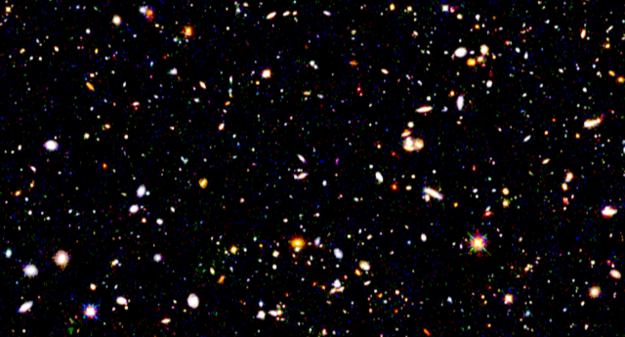
\includegraphics[width=0.5\textwidth]{ESA_Euclid_EDFF_Candels_v1_zoom_625}
    \source{https://sci.esa.int}
  \end{figure}

\end{frame}


%%%%%%%%%%%%%%%%%%%%%%%%%%%%%%%%%%%%
\begin{frame}{Anomalous images or anomalies within images?}

  \begin{itemize}
  \item When looking for anomalous images, we do not necessarily want to detect the source of the anomaly
  \item When an anomaly is detected within an image, then the image is considered as anomalous
  \end{itemize}

\end{frame}


%%%%%%%%%%%%%%%%%%%%%%%%%%%%%%%%%%%%
\begin{frame}{Vocabulary}

  \begin{itemize}
  \item Anomaly
  \item Novelty
  \item Outlier
  \end{itemize}

  In machine learning:

\begin{itemize}
\item One-class classification
\item Out-of-distribution (OOD) detection
\end{itemize}

\end{frame}


%%%%%%%%%%%%%%%%%%%%%%%
%%%%%%%%%%%%%%%%%%%%%%%
\section{Mathematical modeling}

%%%%%%%%%%%%%%%%%%%%%%%%%%%%%%%%%%%%
\begin{frame}{Mathematical framework}

\begin{figure}[ht]
  \centering
  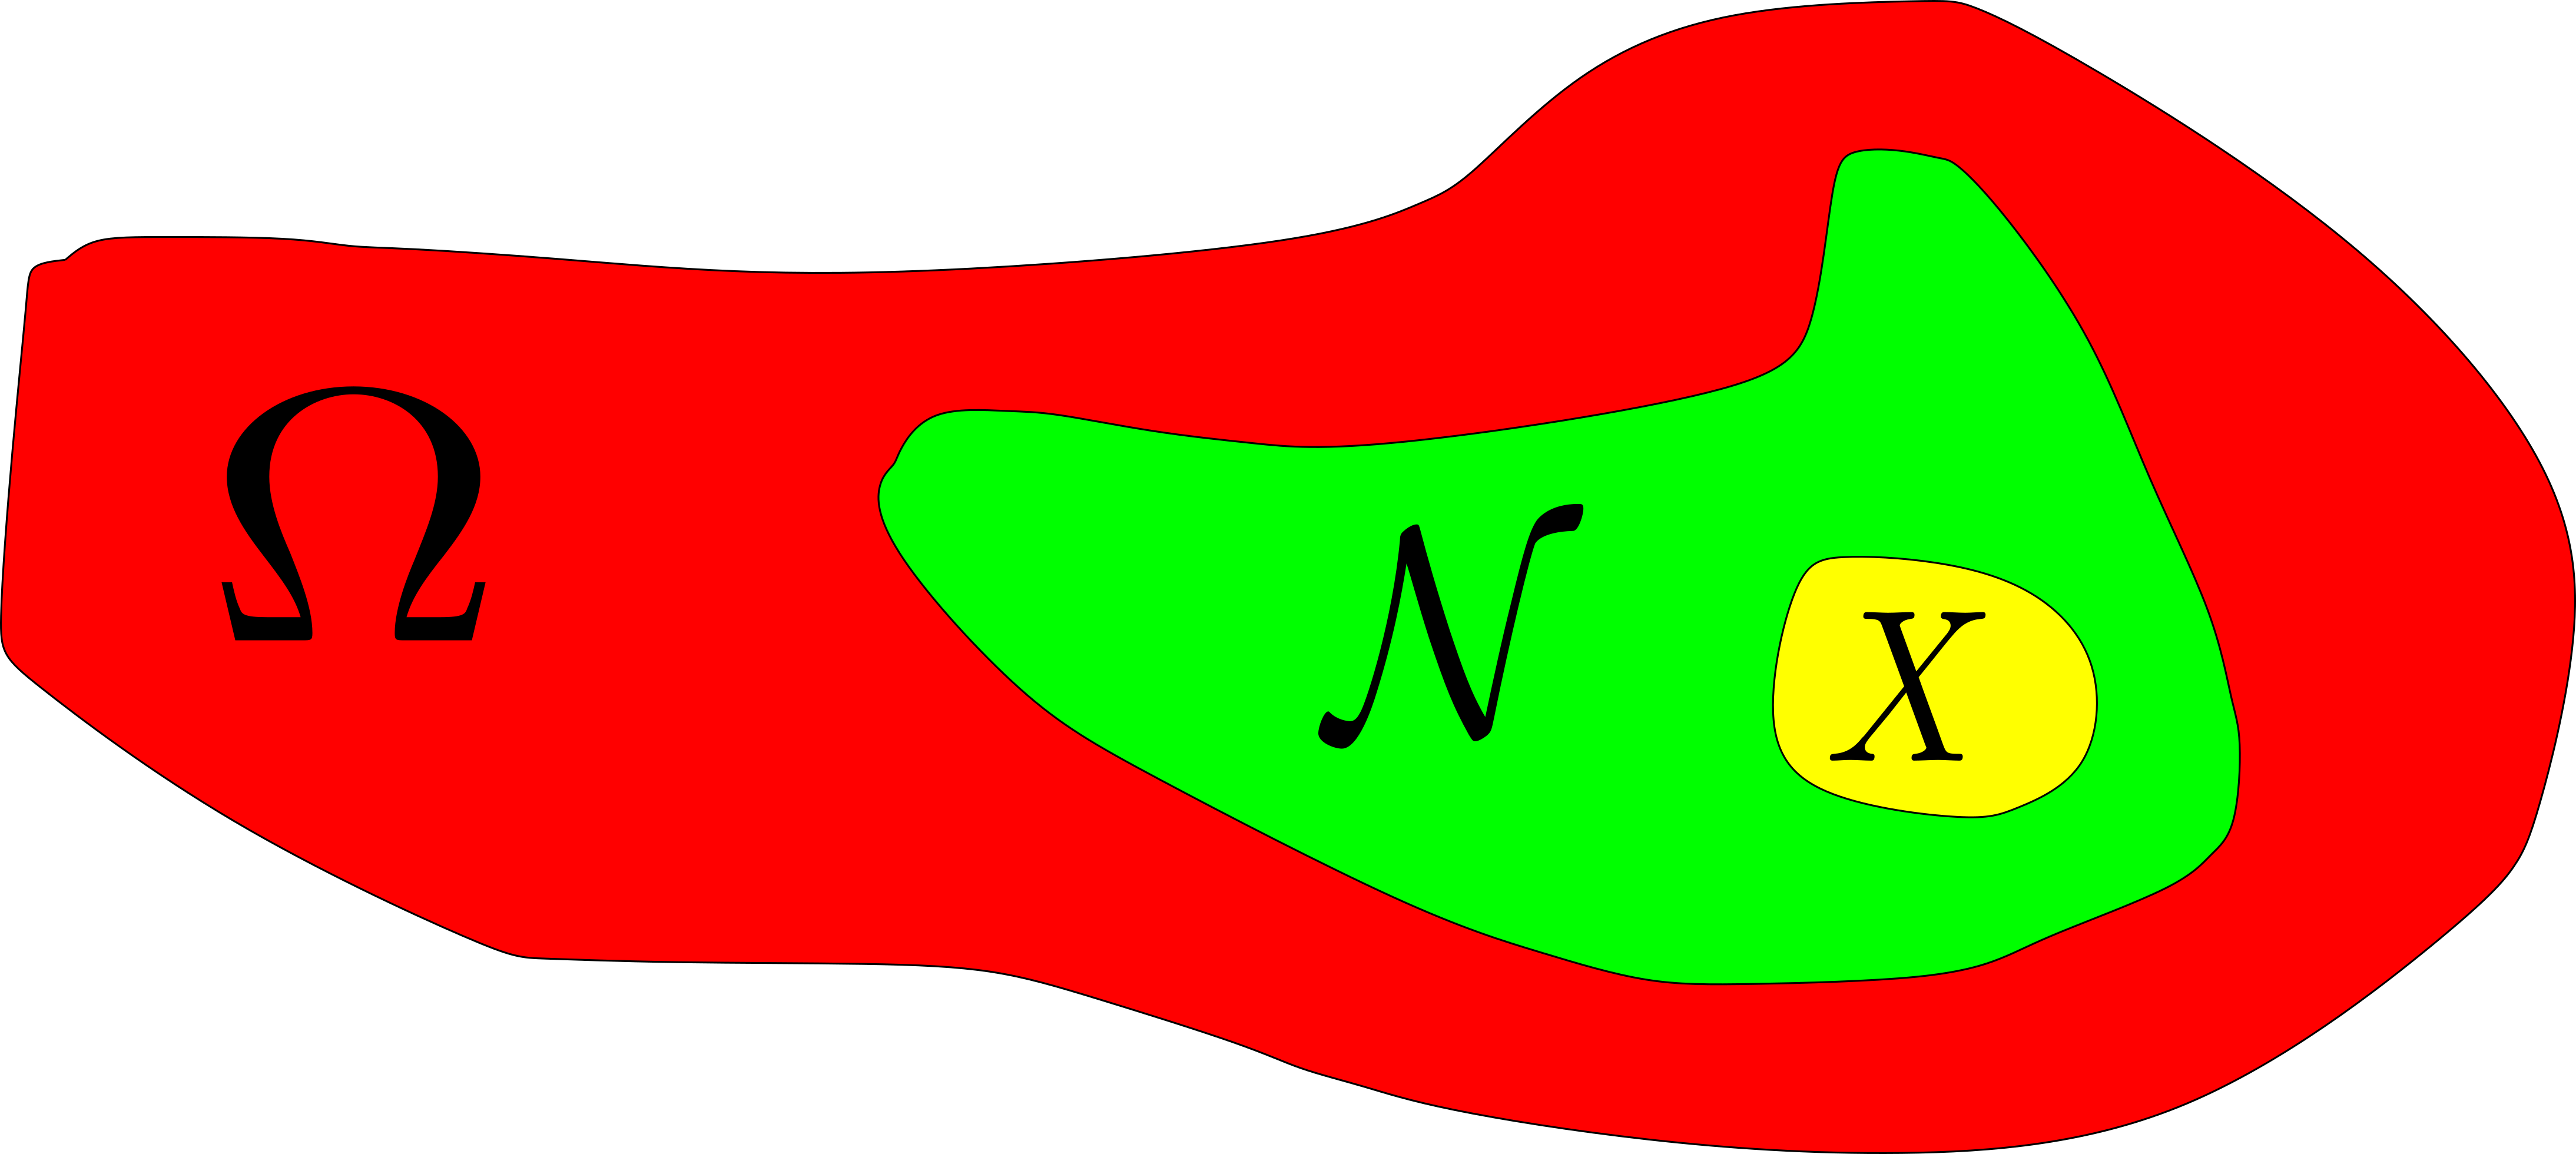
\includegraphics[width=0.5\textwidth]{sets}
\end{figure}


  \begin{block}{Definition}
\begin{itemize}
  \item $\Omega$: a set (the whole set of images)
  \item $\mathcal{N}$: a subset of $\Omega$ (constituted by all normal images)
  \item $X$: a subset of $\mathcal{N}$ (a set of known examples that are considered to be \emph{normal}, i.e. the \alert{training set}).
\end{itemize}
  \end{block}

\end{frame}


%%%%%%%%%%%%%%%%%%%%%%%%%%%%%%%%%%%%
\begin{frame}{Mathematical framework}

\begin{figure}[ht]
  \centering
  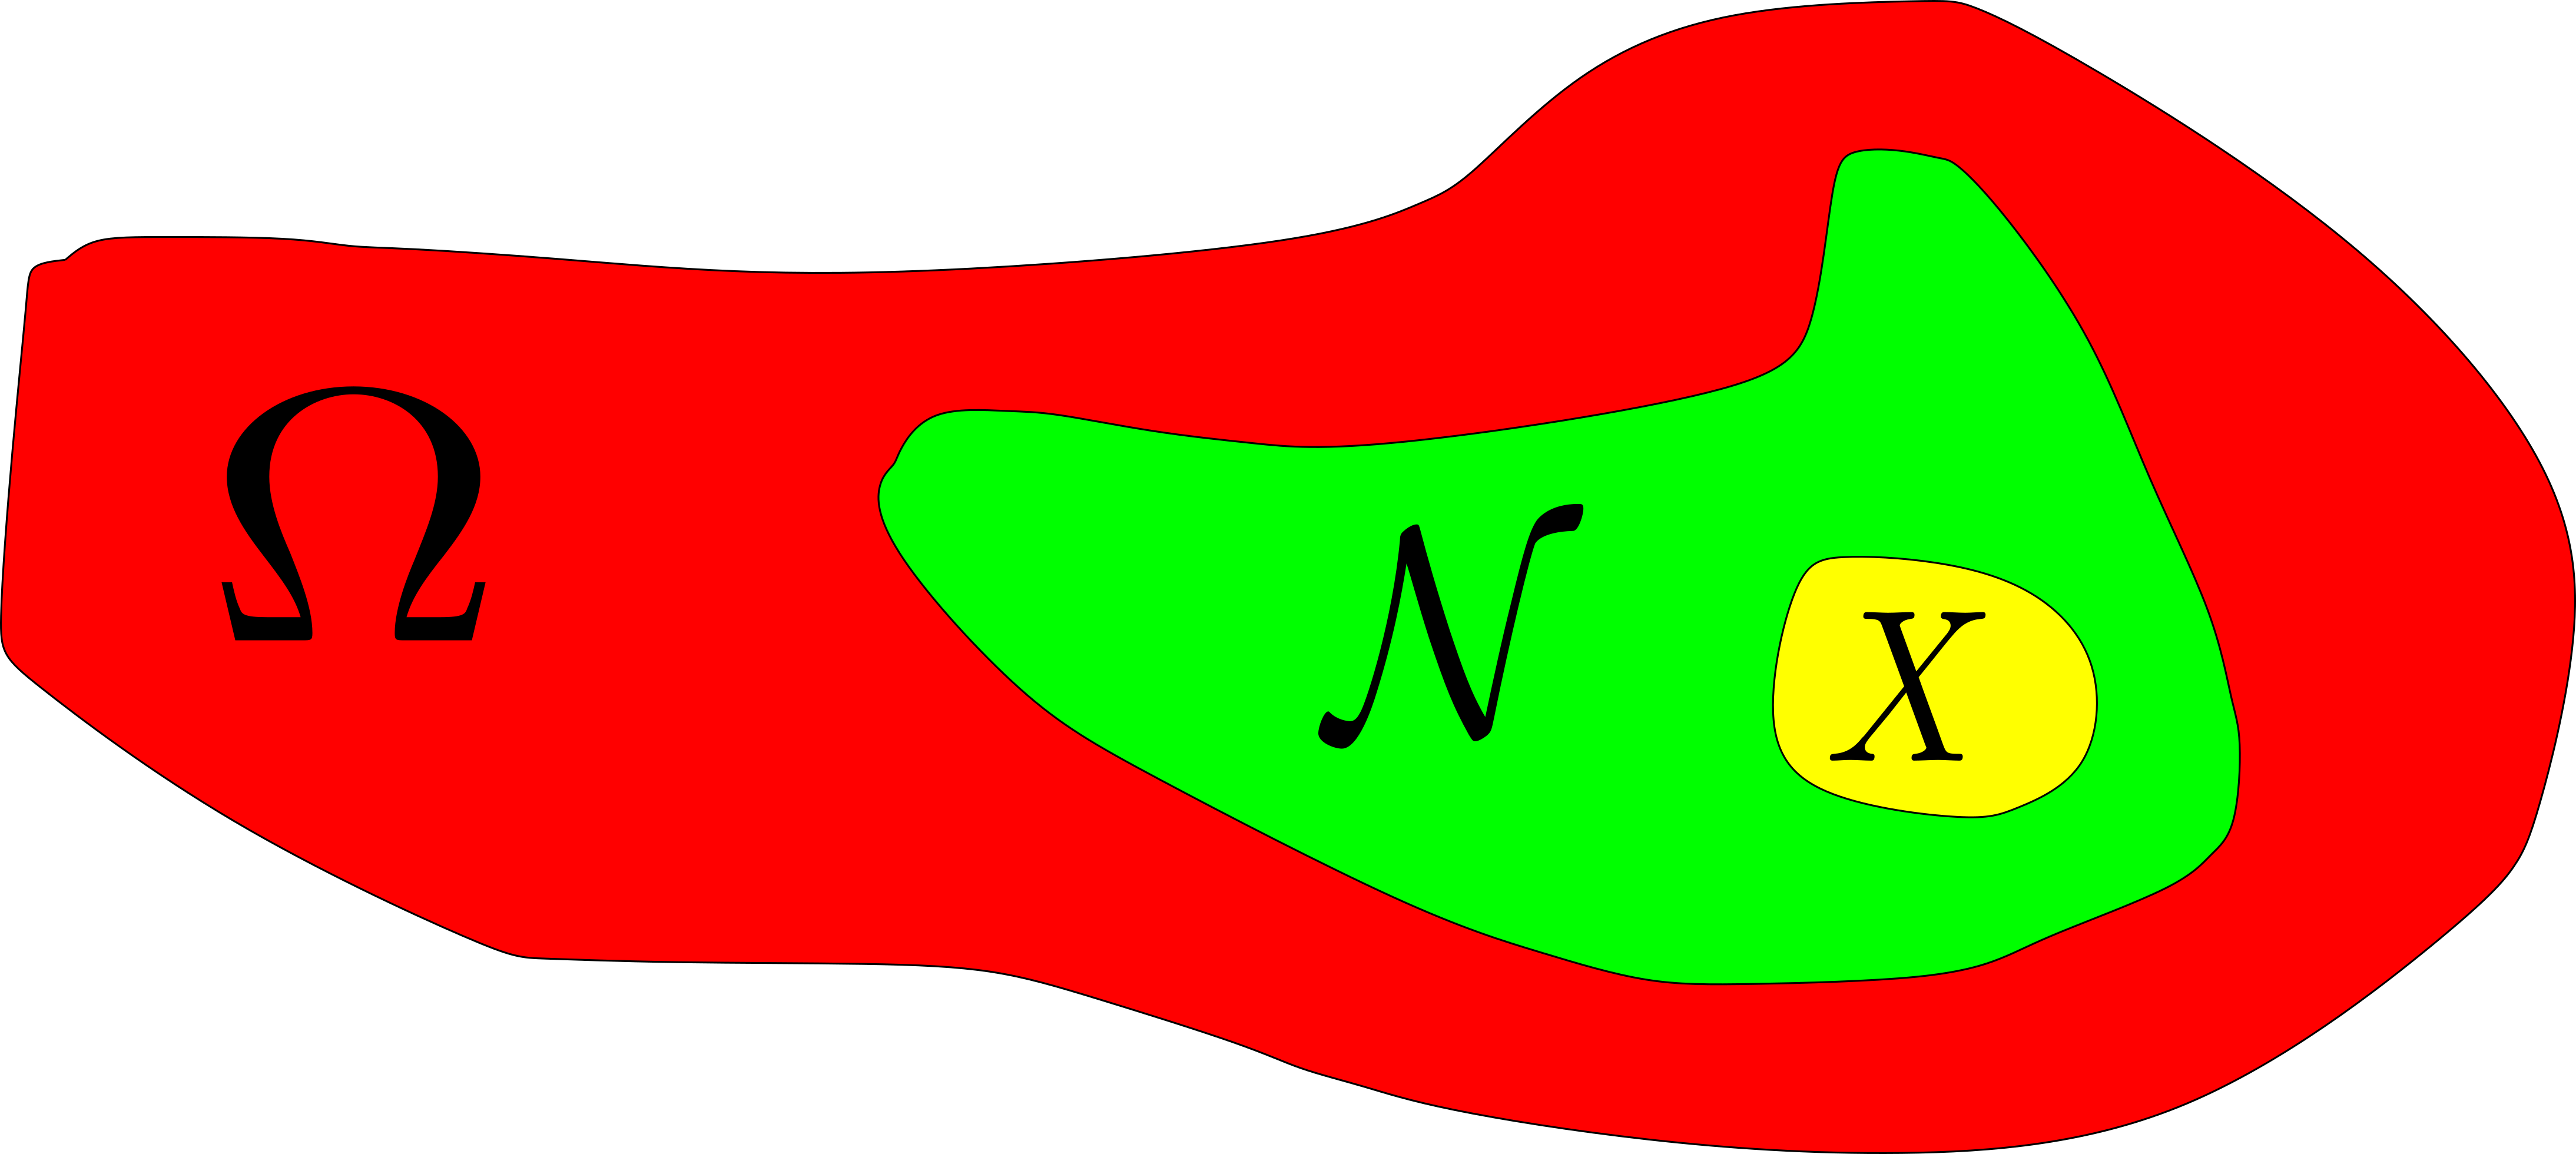
\includegraphics[width=0.5\textwidth]{sets}
\end{figure}


\begin{alertblock}{This graphical representation is misleading}

\begin{itemize}
\item If we equip our set with some kind of topology, there is hardly any reason for $\mathcal{X}$ or $\mathcal{N}$ to be connected. For $\Omega$ connection could be application dependant...
\item We do not know anything about the relative sizes of the sets.
\end{itemize}

\end{alertblock}

\end{frame}


%%%%%%%%%%%%%%%%%%%%%%%%%%%%%%%%%%%%
\begin{frame}{Mathematical framework}

\begin{figure}[ht]
  \centering
  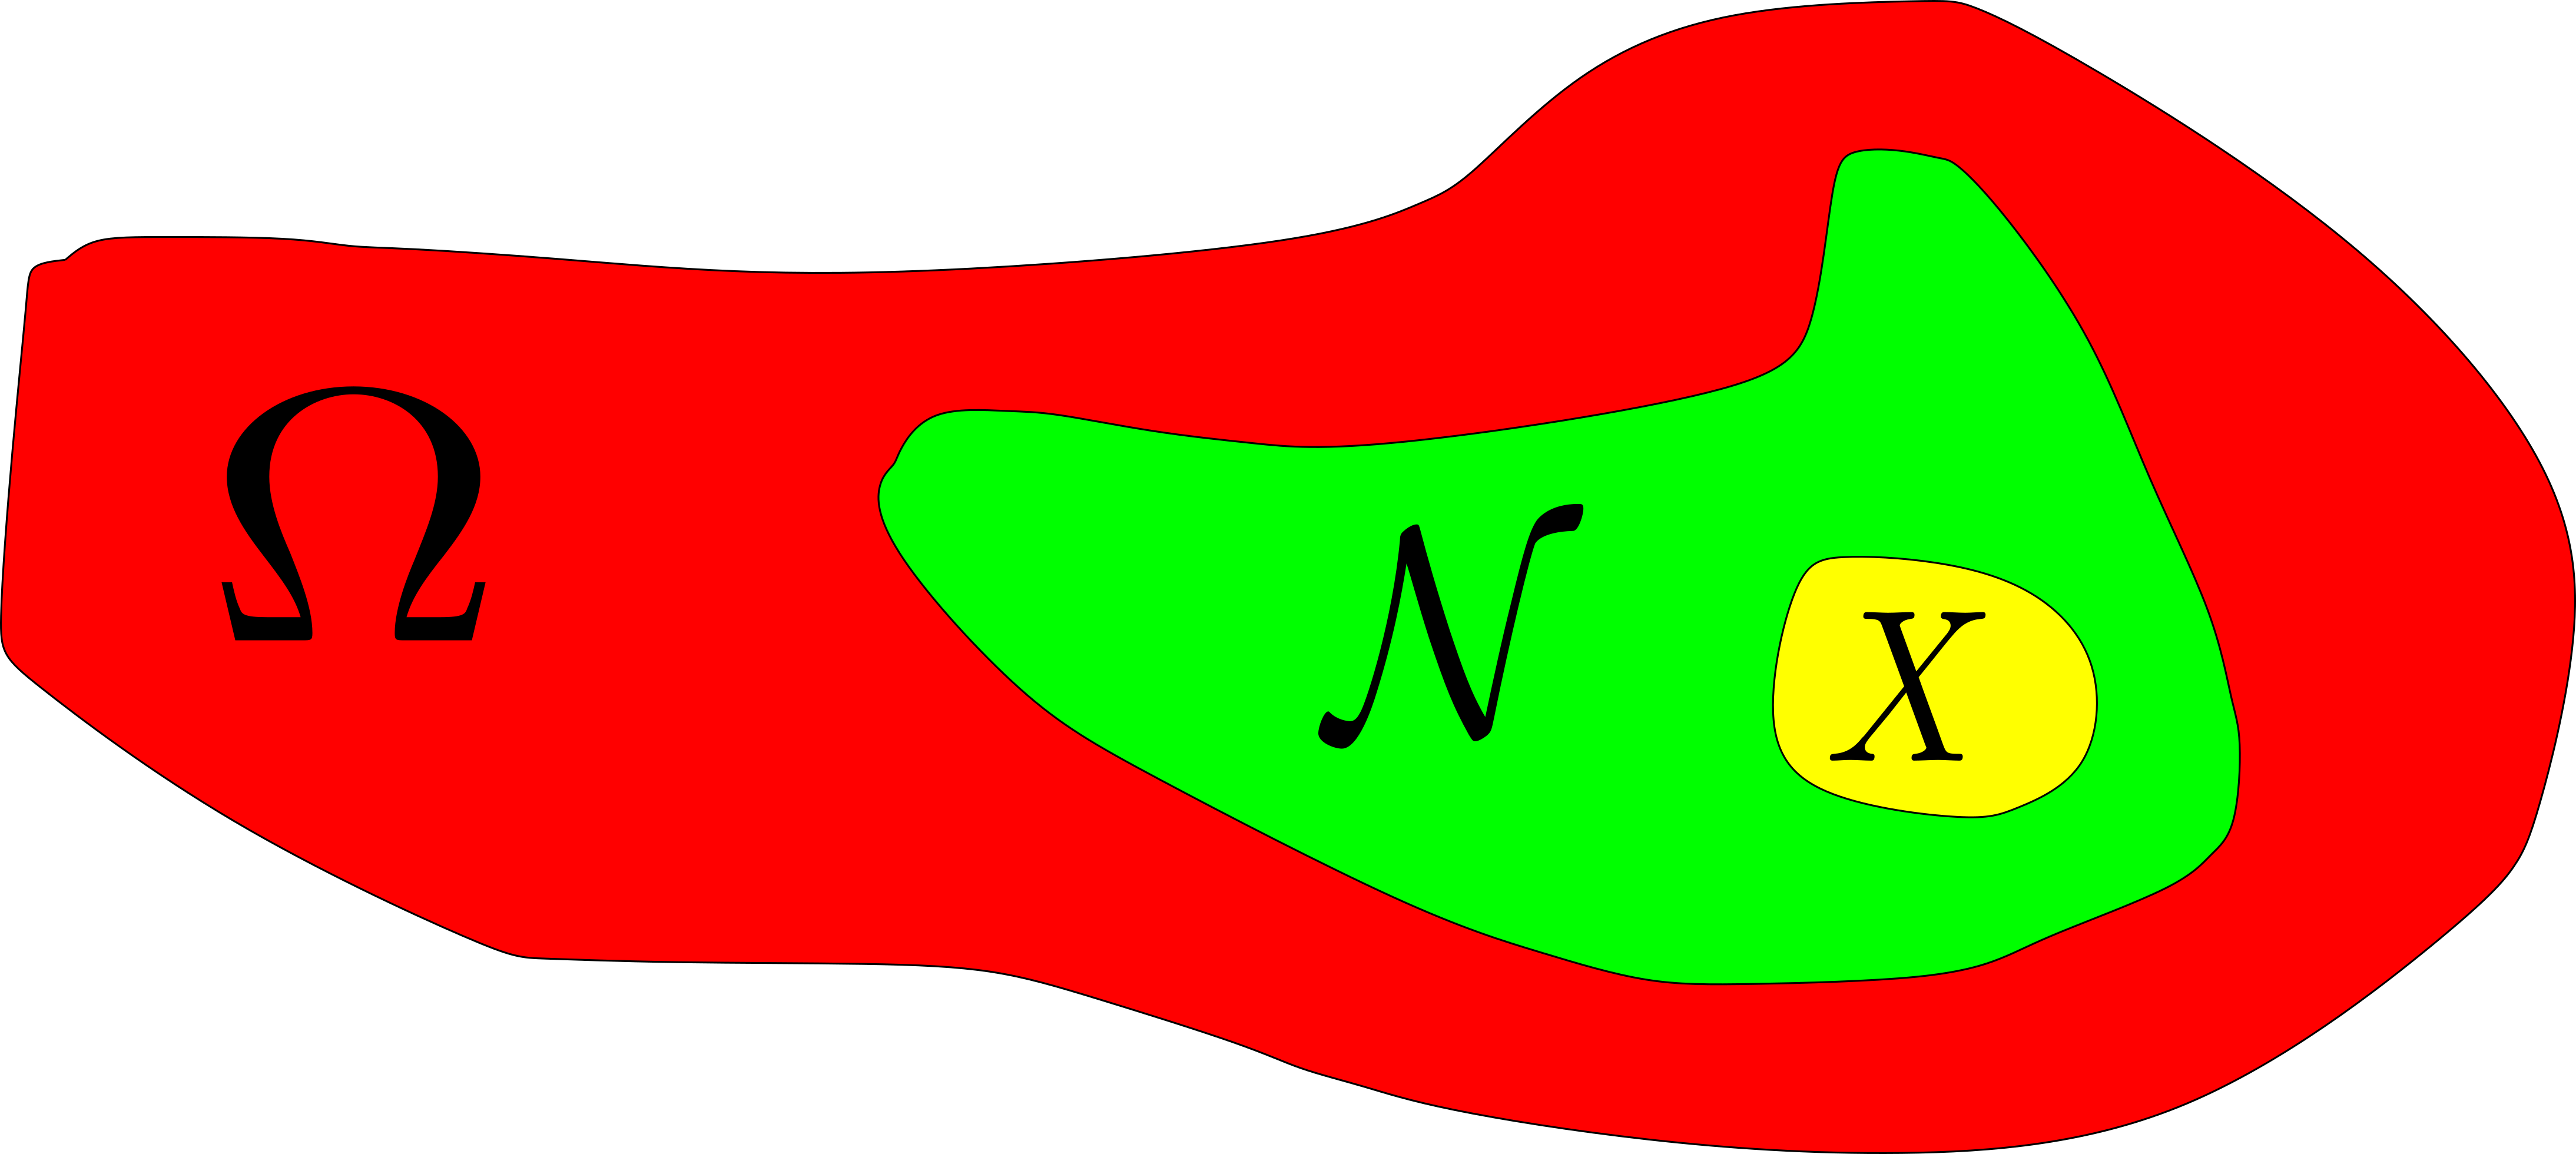
\includegraphics[width=0.5\textwidth]{sets}
\end{figure}



    Some possibilities:
  \begin{itemize}
  \item Explicit modeling of normal images
  \item Generative approach
  \item Probabilistic approach
  \item Metric space
  \end{itemize}

\end{frame}






%%%%%%%%%%%%%%%%%%%%%%%%%%%%%%%%%%%%
\begin{frame}{Explicit modeling}

  If a mathematical model can be hand-crafted to describe normal images, then it can be used to detect abnormal ones.

  \begin{block}{Suspicious object or unusual behaviour in a scene}
    \begin{figure}[ht]
      \centering
      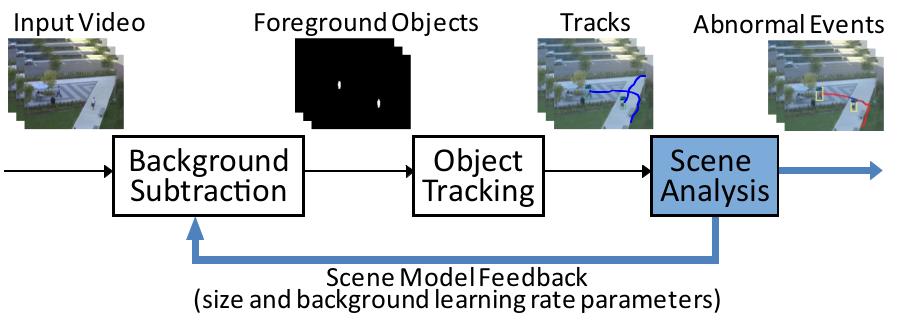
\includegraphics[width=\textwidth]{motion_patterns_anom_det}
      \source{\cite{basharat_learning_2008}}
    \end{figure}

  \end{block}

\end{frame}

%%%%%%%%%%%%%%%%%%%%%%%%%%%%%%%%%%%%
\begin{frame}{Generative approach}

  \begin{block}{Idea}
    Normal images are considered as the result of some generation function $G$.
    \[
    \begin{split}
    G: & ~~~~\mathcal{Z} \longrightarrow \mathcal{N} \\
    & ~~~~ z \longmapsto G(z)
    \end{split}
    \]
  \end{block}

\begin{itemize}
\item In practice we will also need the \emph{encoding} function $E$:
    \[
    \begin{split}
    E: & ~~~~\mathcal{N} \longrightarrow \mathcal{Z} \\
    & ~~~~ \x \longmapsto E(\x)
    \end{split}
    \]
\end{itemize}

\end{frame}


%%%%%%%%%%%%%%%%%%%%%%%%%%%%%%%%%%%%
\begin{frame}{Probabilistic approach}

This can be considered as a generalization of the previous approach.

\begin{block}{Idea}

  \begin{itemize}
  \item   The images of $\Omega$ are considered as the realization of some random process (i.e. \emph{random images}). A probability can therefore be associated to each image.
  \item Normal images are those whose associated probability is \emph{high enough}
  \end{itemize}

\end{block}



\end{frame}



%%%%%%%%%%%%%%%%%%%%%%%%%%%%%%%%%%%%
\begin{frame}{Metric space}

  The aim is to equip $\Omega$ with a distance $d$ such that:
  \[
  \exists d_0 \in \R^+,  \forall x \in \Omega: x \in \mathcal{N} \iff d(x, X) \leq d_0
  \]

  Of course, the essential point will be how to choose the distance function $d$.


%% \begin{block}{Mahalanobis distance}
%%   A distance function that takes into account the distribution of the data.
%% \end{block}

\end{frame}


%%%%%%%%%%%%%%%%%%%%%%%%%%%%%%%%%%%%
%% \begin{frame}{Energy based approach}

%% \end{frame}

%%%%%%%%%%%%%%%%%%%%%%%%%%%%%%%%%%%%
\begin{frame}{Representing images}

  \begin{block}{Trivial representation}
    A 2D grey level image is a real array of size $p \times q$.
  \end{block}

  \begin{itemize}
  \item Classical distances between arrays ($L_2, L_1, \ldots$) do not make sense from a semantic point of view
  \end{itemize}

\begin{columns}
  \begin{column}{.5\textwidth}
  \begin{figure}[ht]
    \centering
    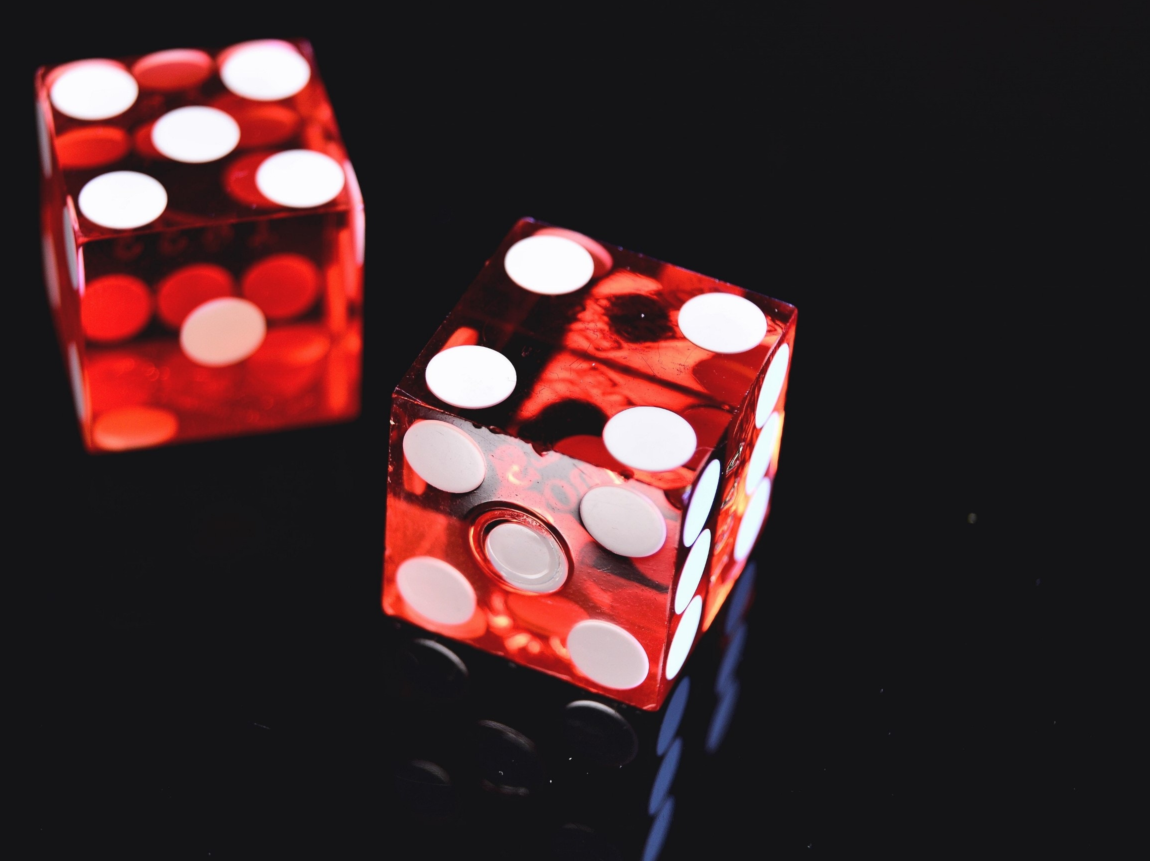
\includegraphics[width=0.8\textwidth]{pexels-jonathan-petersson-965875-1}
  \end{figure}

  \end{column}

  \begin{column}{.5\textwidth}
  \begin{figure}[ht]
    \centering
    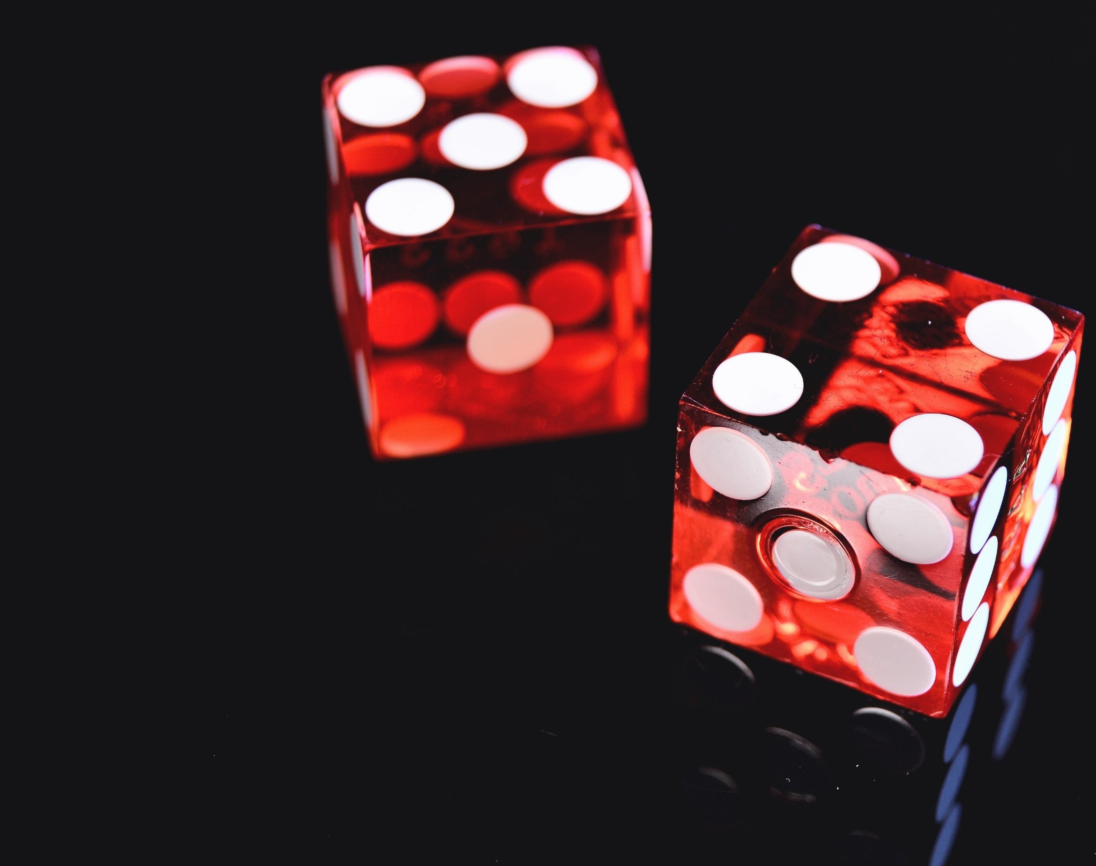
\includegraphics[width=0.78\textwidth]{pexels-jonathan-petersson-965875-2}
  \end{figure}

  \end{column}
\end{columns}
    \source{Jonathan Petersson on pexels.com}


\end{frame}

%%%%%%%%%%%%%%%%%%%%%%%%%%%%%%%%%%%%
\begin{frame}{Representing images}

\begin{block}{}
  Finding a good image representation, where typically perceptual distances can be easily computed, is an important research topic.
\end{block}

    \[
    \begin{split}
    E: & ~~~~\Omega \longrightarrow \mathcal{Z} \\
    & ~~~~ \x \longmapsto E(\x)
    \end{split}
    \]

\end{frame}



%%%%%%%%%%%%%%%%%%%%%%%%%%%%%%%%%%%%%%%%%%%%%%%%%%
%%%%%%%%%%%%%%%%%%%%%%%%%%%%%%%%%%%%%%%%%%%%%%%%%%
\section{Anomaly detection using autoencoders}


%%%%%%%%%%%%%%%%%%%%%%%%%%%%%%%%%%%%
\begin{frame}{Autoencoder}

  \begin{figure}[ht]
    \centering
    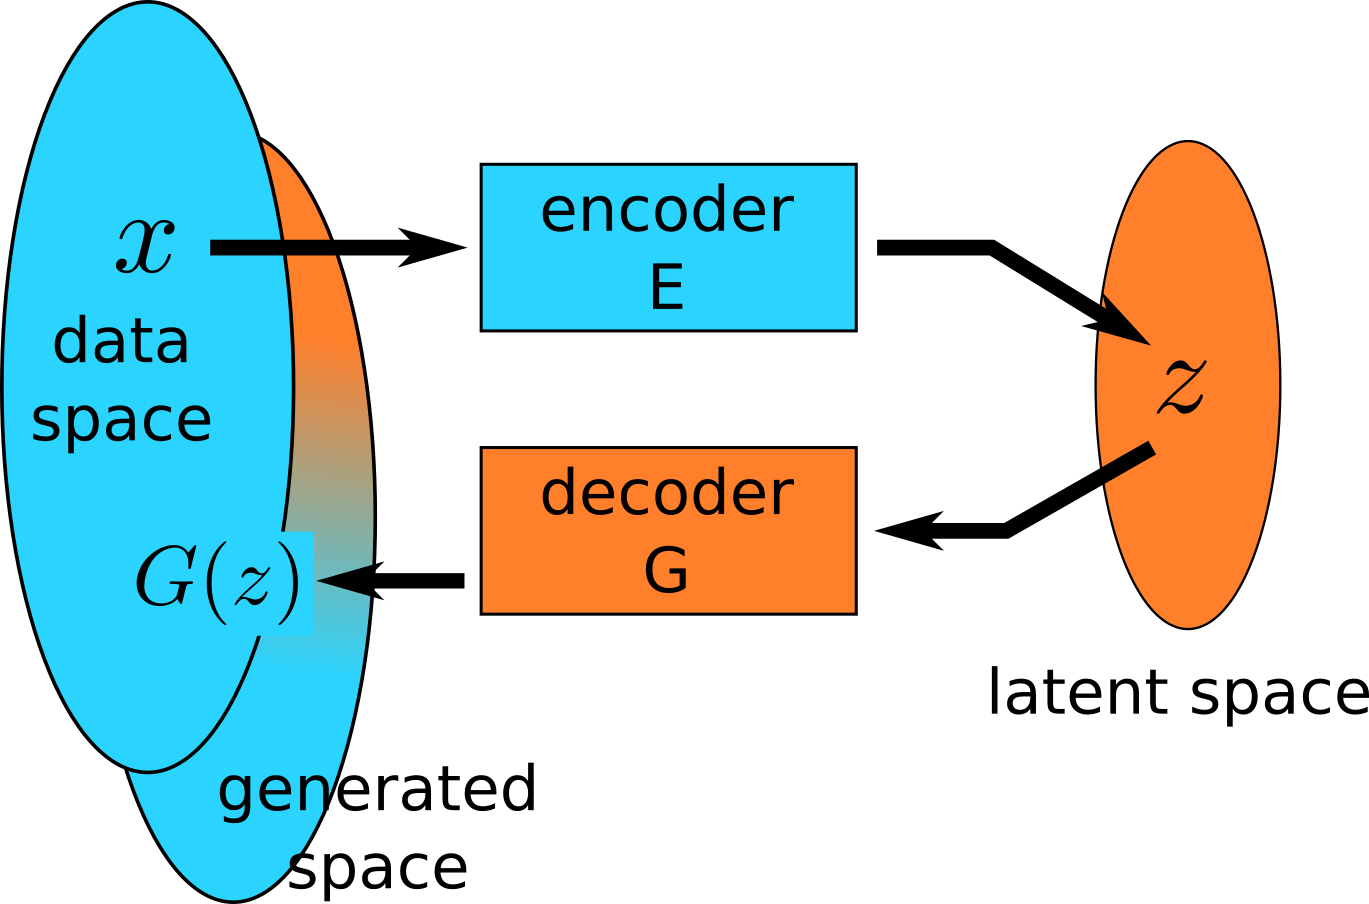
\includegraphics[width=0.5\textwidth]{ae.png}
  \end{figure}

  \begin{itemize}
  \item Encoder: $E$; decoder: $G$; autoencoder: $G \circ E$
  \item In most applications, the latent space is ``smaller'' than the data space.
  \item Objective: $G(E(x))$ ``close'' to $x$
  \item When dealing with images, modern autoencoders use convolutional neural networks
  \end{itemize}

\end{frame}

%%%%%%%%%%%%%%%%%%%%%%%%%%%%%%%%%%%%
\begin{frame}{Autoencoders for anomalous image detection}

  \begin{figure}[ht]
    \centering
    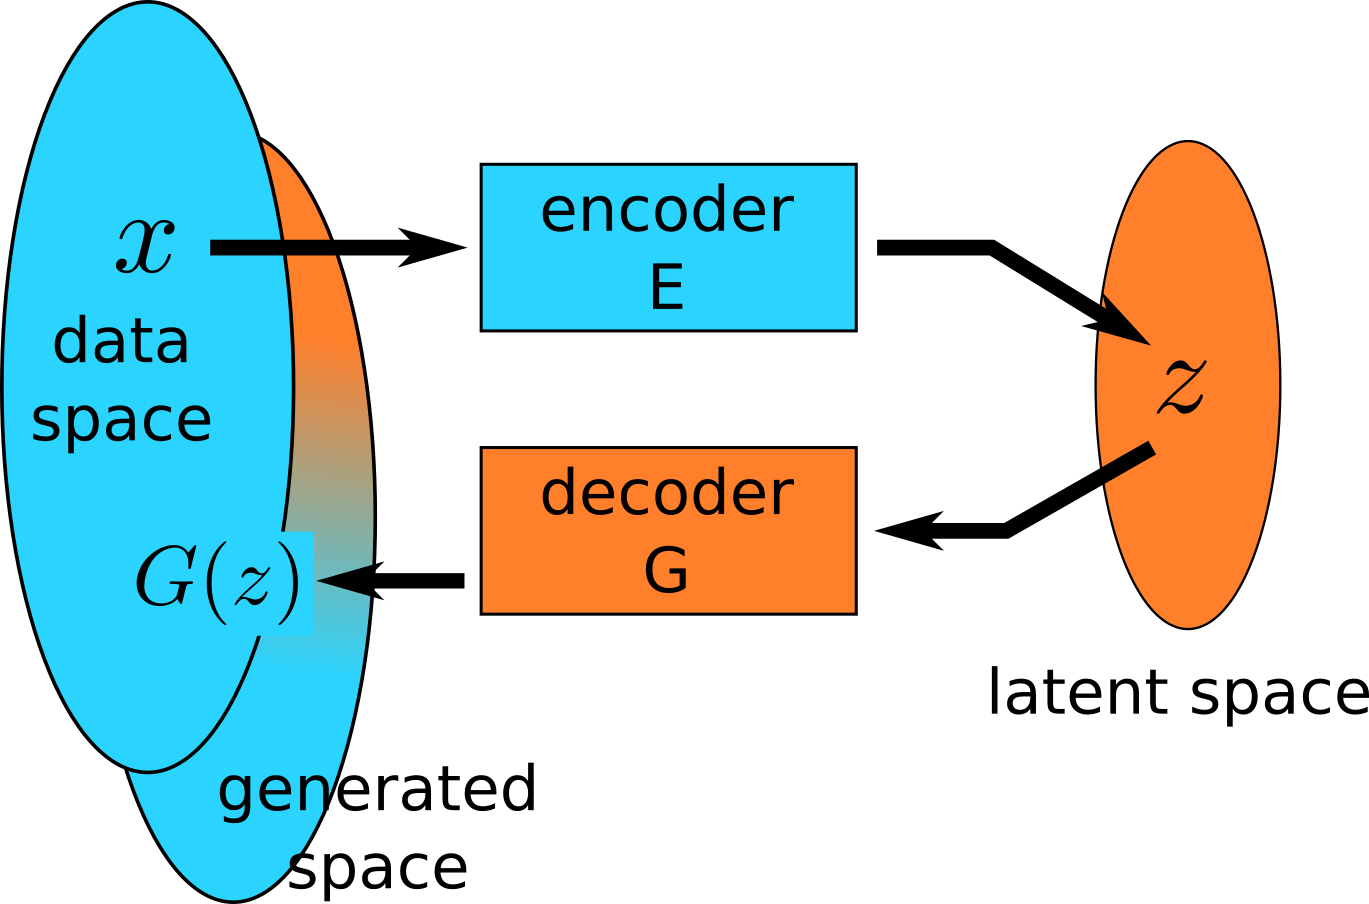
\includegraphics[width=0.5\textwidth]{ae.png}
  \end{figure}

  \begin{block}{Idea 1}
    The autoencoders is optimized for normal images. The coding has to be specific enough so that anomalous images are not correctly coded. The reconstruction error will therefore give a measure of the anomaly.
  \end{block}

\end{frame}

%%%%%%%%%%%%%%%%%%%%%%%%%%%%%%%%%%%%
\begin{frame}{Autoencoders for anomalous image detection}

  \begin{figure}[ht]
    \centering
    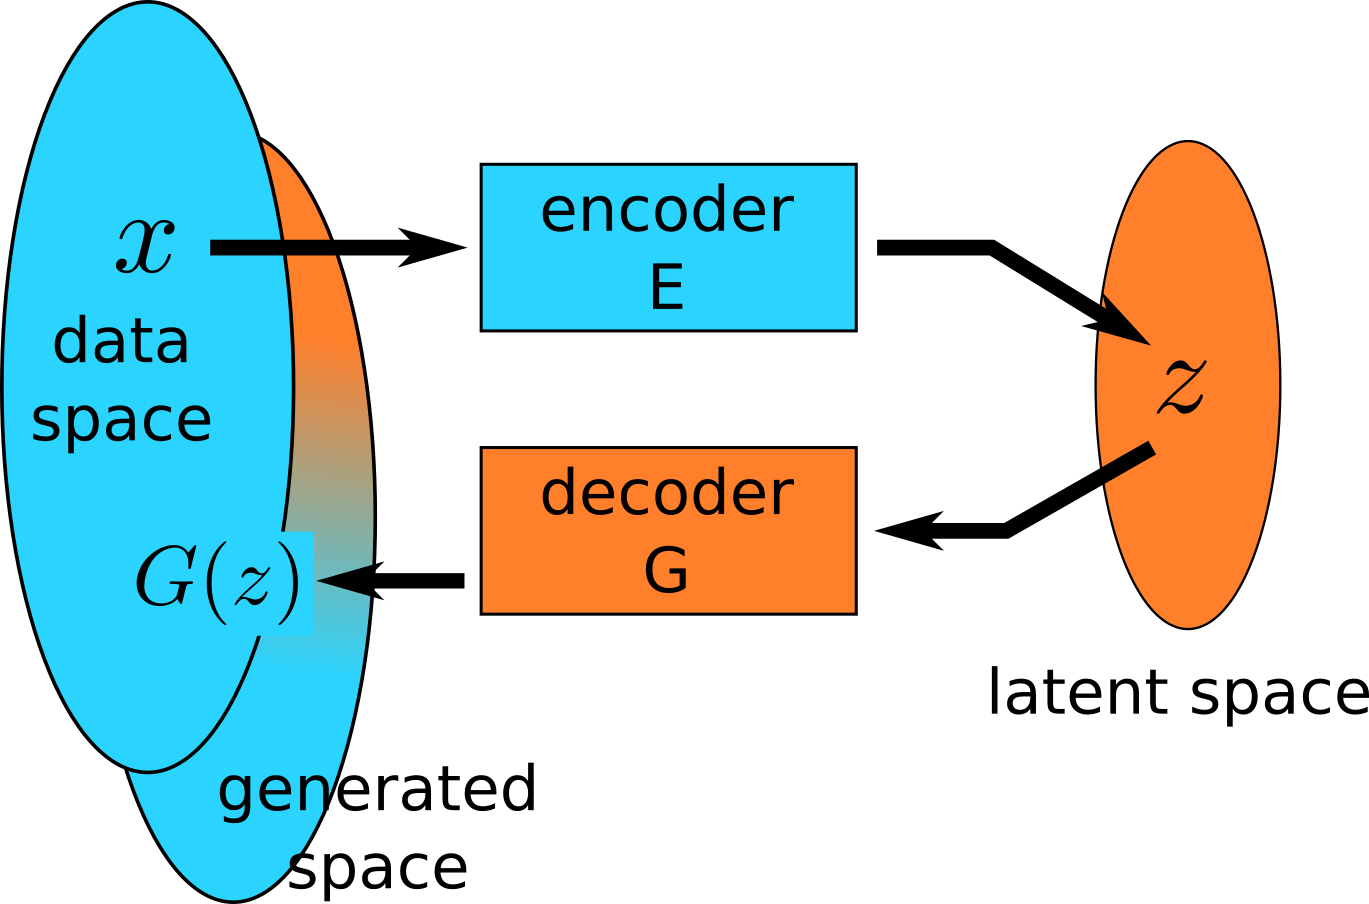
\includegraphics[width=0.5\textwidth]{ae.png}
  \end{figure}

  \begin{block}{Idea 2}
    The latent representation of an anomalous image should be ``far away'' from the latent representations of normal images. Image $\x$ is not normal iff $d(E(\x), E(\X)) > d_0$.
  \end{block}

\end{frame}

%%%%%%%%%%%%%%%%%%%%%%%%%%%%%%%%%%%%
\begin{frame}{Conclusion on autoencoders for anomaly detection}

  \begin{itemize}
  \item Understanding the failure of reconstruction-based approaches is important. Using a perceptual distance might be an interesting approach.
  \item In practice, methods based on the latent space seem to give the best results.
  \item Are there ways to find a better image representation?
  \end{itemize}

\end{frame}


%%%%%%%%%%%%%%%%%%%%%%%%%%%%%%%%%%%%%%%%%%%%%%%%%%
%%%%%%%%%%%%%%%%%%%%%%%%%%%%%%%%%%%%%%%%%%%%%%%%%%
\section{Anomaly detection using generative adversarial networks (GANS)}

%%%%%%%%%%%%%%%%%%%%%%%%%%%%%%%%%%%%
\begin{frame}{Generative adversarial network \cite{goodfellow_generative_2014}}

  \begin{figure}[ht]
    \centering
    \includegraphics[width=0.6\textwidth]{gan2}
  \end{figure}

  \begin{itemize}
  \item The discriminator is optimized so that it correctly classifies images as real (1) or fake (0)
  \item The generator is optimized so that the produced images are classified as real by the discriminator
  \end{itemize}

  \begin{block}{Value function}
    $V(G,D) = \mathbb{E}_{p_\x}(log(D(\x))) + \mathbb{E}_{p_z(z)}(log(1 - D(G(z))))$
  \end{block}

\end{frame}


%%%%%%%%%%%%%%%%%%%%%%%%%%%%%%%%%%%%
\begin{frame}{First application of GANs to novelty detection}

  \begin{block}{Idea}
    Use the discriminator to distinguish between real and fake images.
  \end{block}

  \begin{itemize}
  \item I have seen no mention of this strategy in the literature
  \item My guess: the discriminator is not very efficient at this task.
  \end{itemize}

\end{frame}


%%%%%%%%%%%%%%%%%%%%%%%%%%%%%%%%%%%%
\begin{frame}{Anomaly GAN (AnoGAN) \cite{schlegl_unsupervised_2017}}

  \begin{figure}[ht]
    \centering
    \includegraphics[width=0.6\textwidth]{gan2}
  \end{figure}

  \begin{enumerate}
  \item Learn a GAN on the set of normal images
  \item For a new image $\x$ (normal or not):
    \begin{itemize}
    \item Find a $z^*$ such that $G(z^*)$ is \emph{close as possible} to $\x$
    \item If $G(z^*)$ is \emph{similar enough} to $\x$ and is \emph{correctly evaluated by the descriminator}, then $\x$ is considered as normal
    \end{itemize}
  \end{enumerate}

\end{frame}

%%%%%%%%%%%%%%%%%%%%%%%%%%%%%%%%%%%%
\begin{frame}{Finding $z^*$}

  \begin{figure}[ht]
    \centering
    \includegraphics[width=0.4\textwidth]{gan2}
  \end{figure}

  We have $G$, but not $G^{-1}$.

  \begin{itemize}
  \item For a given $\x$, a random $z_0$ is sampled from the latent space $\cal{Z}$
  \item A loss function $\mathcal{L}$ is defined to evaluate the fitness of any $z$ with respect to $\x$
  \item With the network parameters fixed, backpropagation is used to obtain $(z_i)$ starting from $z_0$. The last $z_i$ is considered as the best: $z^*$.
  \end{itemize}

\end{frame}


%%%%%%%%%%%%%%%%%%%%%%%%%%%%%%%%%%%%
\begin{frame}{Is $\x$ similar to $G(z_i)$ ?}

  \begin{figure}[ht]
    \centering
    \includegraphics[width=0.4\textwidth]{gan2}
  \end{figure}

  \begin{block}{Residual loss}
    \centering
    $\mathcal{L}_R(z_i) = \norm{x - G(z_i)}_{L_1}$
  \end{block}

\end{frame}


%%%%%%%%%%%%%%%%%%%%%%%%%%%%%%%%%%%%
\begin{frame}{Is $G(z_i)$ realistic?}

  \begin{figure}[ht]
    \centering
    \includegraphics[width=0.4\textwidth]{gan2}
  \end{figure}

  \begin{block}{Discrimination loss}
    \centering
    $\mathcal{L}_D(z_i) = D(G(z_i))$
  \end{block}

  \begin{block}{Improved discrimination loss}
    \[\mathcal{L}_D(z_i) = \norm{f_D(\x) - f_D(G(z_i))}_{L_1}\]
    where $f_D$ is the last layer of the discriminator.
  \end{block}


\end{frame}


%%%%%%%%%%%%%%%%%%%%%%%%%%%%%%%%%%%%
\begin{frame}{Final loss and anomaly evaluation}

  \begin{block}{Final loss}
    \[\mathcal{L}(z_i) = (1-\alpha)\mathcal{L}_D(z_i) + \alpha \mathcal{L}_R(z_i) \]
  \end{block}

  \begin{block}{Anomaly evaluation}
    \[A(\x) = (1-\alpha)\mathcal{L}_D(z^*) + \alpha \mathcal{L}_R(z^*) \]

      Moreover, the \emph{residual image}:
      \[
      |\x - G(z^*)|
      \]
      is used to detect anomalous regions.
  \end{block}

\end{frame}


%%%%%%%%%%%%%%%%%%%%%%%%%%%%%%%%%%%%
\begin{frame}{Example (from \cite{schlegl_unsupervised_2017})}


  \begin{figure}[ht]
    \centering
    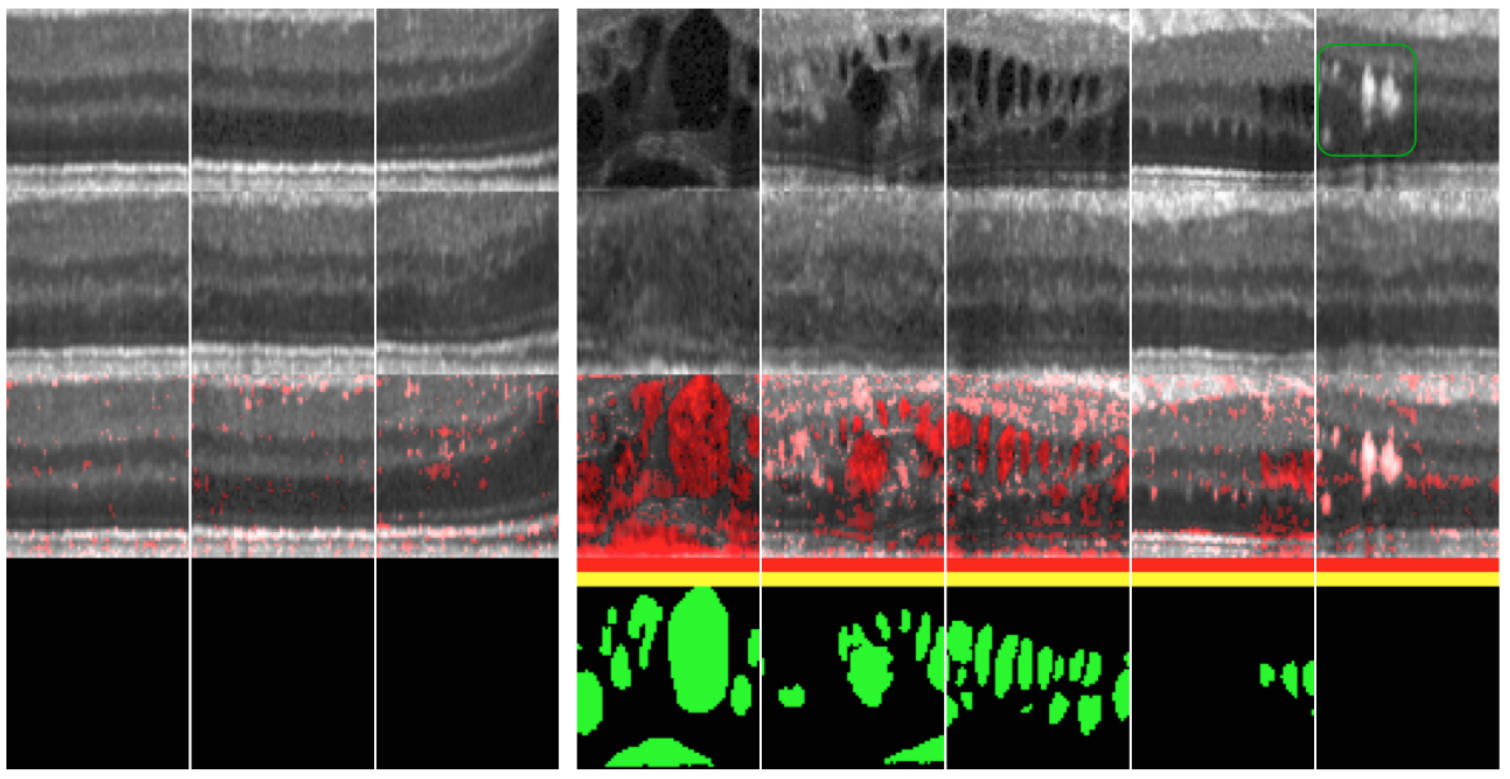
\includegraphics[width=\textwidth]{res_oct}
    \caption*{Left block: normal OCT sections, from test set. Right block: anomalous OCT sections; bottom line: expert annotation of retinal fluid}
  \end{figure}

\end{frame}


%%%%%%%%%%%%%%%%%%%%%%%%%%%%%%%%%%%%
\begin{frame}{AnoGAN improvement}

  \begin{figure}[ht]
    \centering
    \includegraphics[width=0.6\textwidth]{gan2}
  \end{figure}

  \begin{itemize}
  \item For a given real image $\x$, finding a latent code $z$ such that $G(z)$ is similar to $\x$ is computationally intensive
  \item Idea: learn an encoder to compute $z$ from $\x$
  \end{itemize}

\end{frame}

%%%%%%%%%%%%%%%%%%%%%%%%%%%%%%%%%%%%
\begin{frame}{BiGAN}

  \begin{figure}[ht]
    \centering
    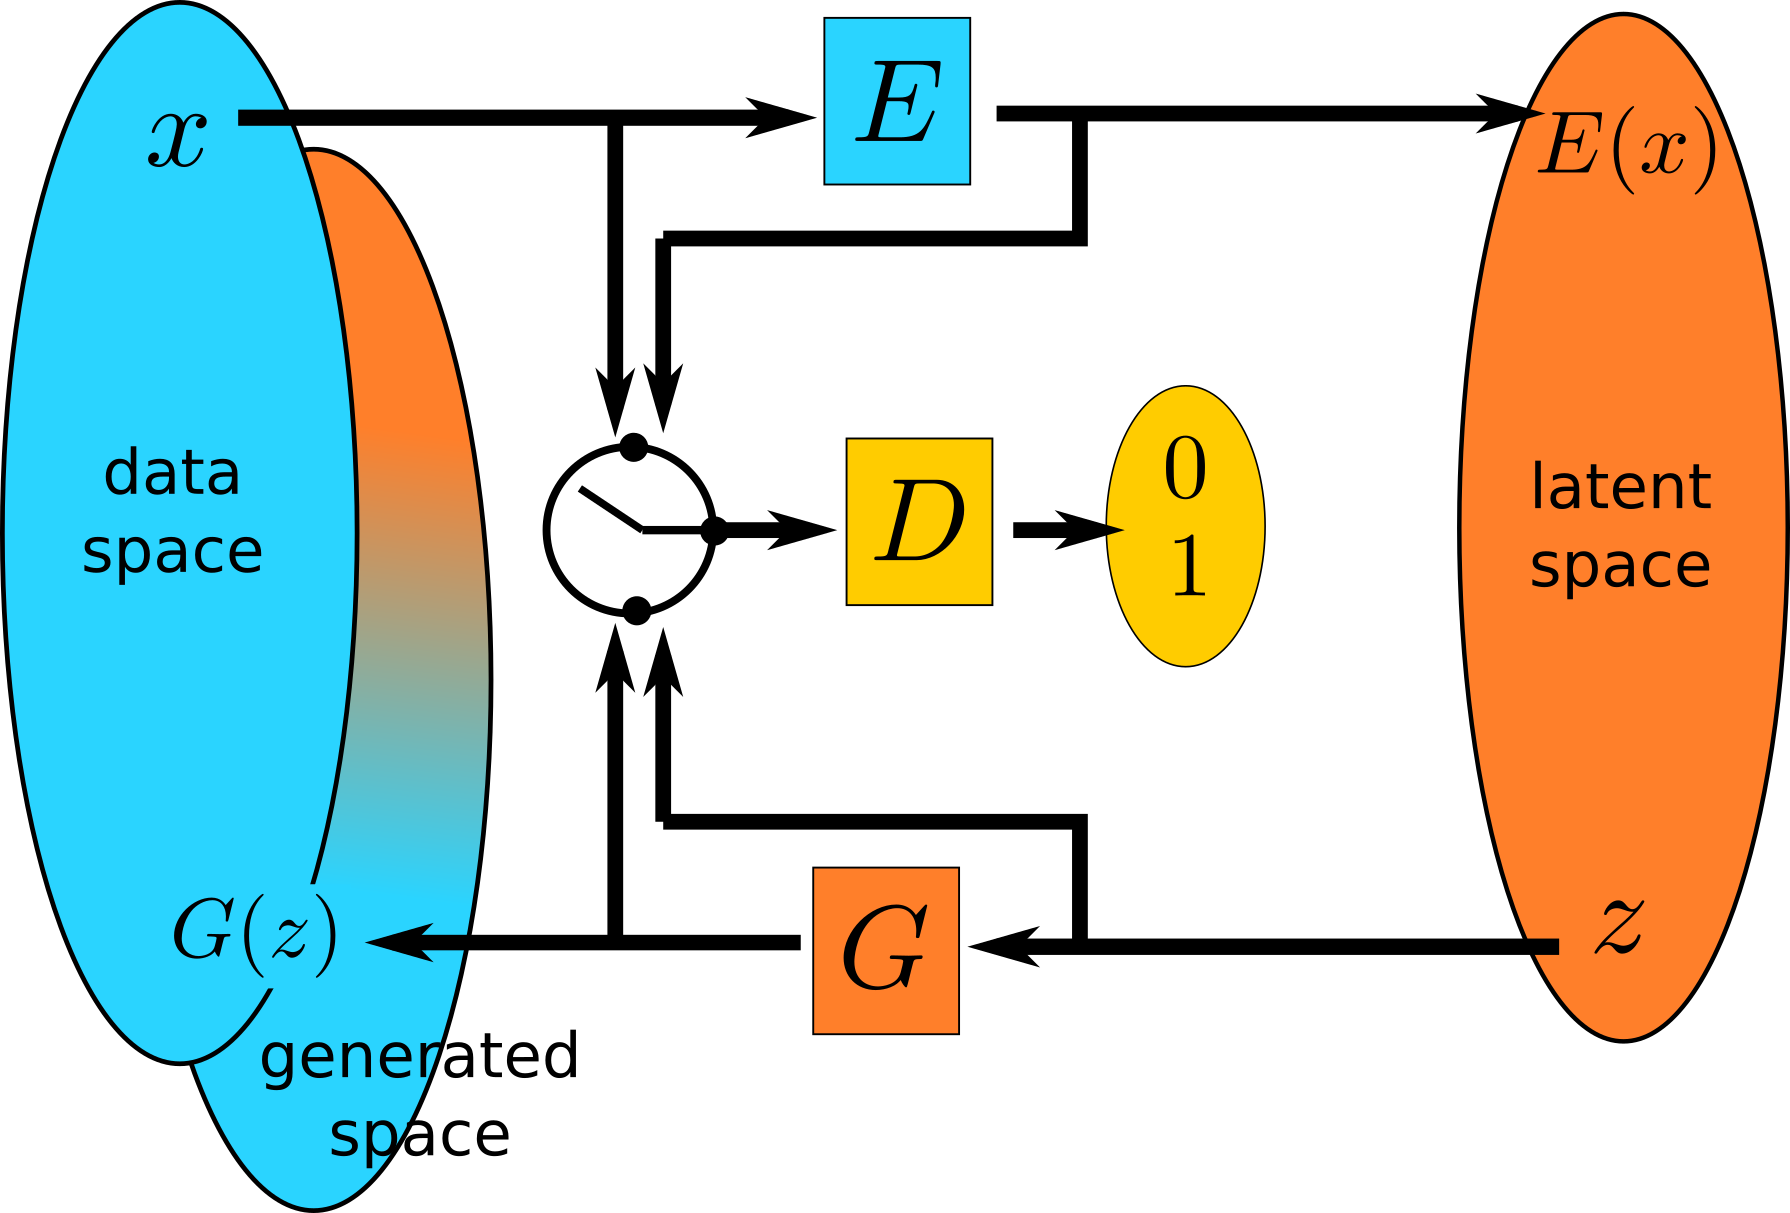
\includegraphics[width=0.6\textwidth]{bigan}
  \end{figure}

  \begin{itemize}
  \item An encoder is added to the architecture
  \item The discriminator takes as input pairs of image / code
  \end{itemize}

    \begin{block}{Value function}
    $V(G,D) = \mathbb{E}_{p_\x}(log(D(\x, E(\x)))) + \mathbb{E}_{p_z(z)}(log(1 - D(G(z), z)))$
  \end{block}


\end{frame}

%%%%%%%%%%%%%%%%%%%%%%%%%%%%%%%%%%%%
\begin{frame}{BiGAN: application to novelty detection \cite{zenati_efficient_2018}}

  \begin{figure}[ht]
    \centering
    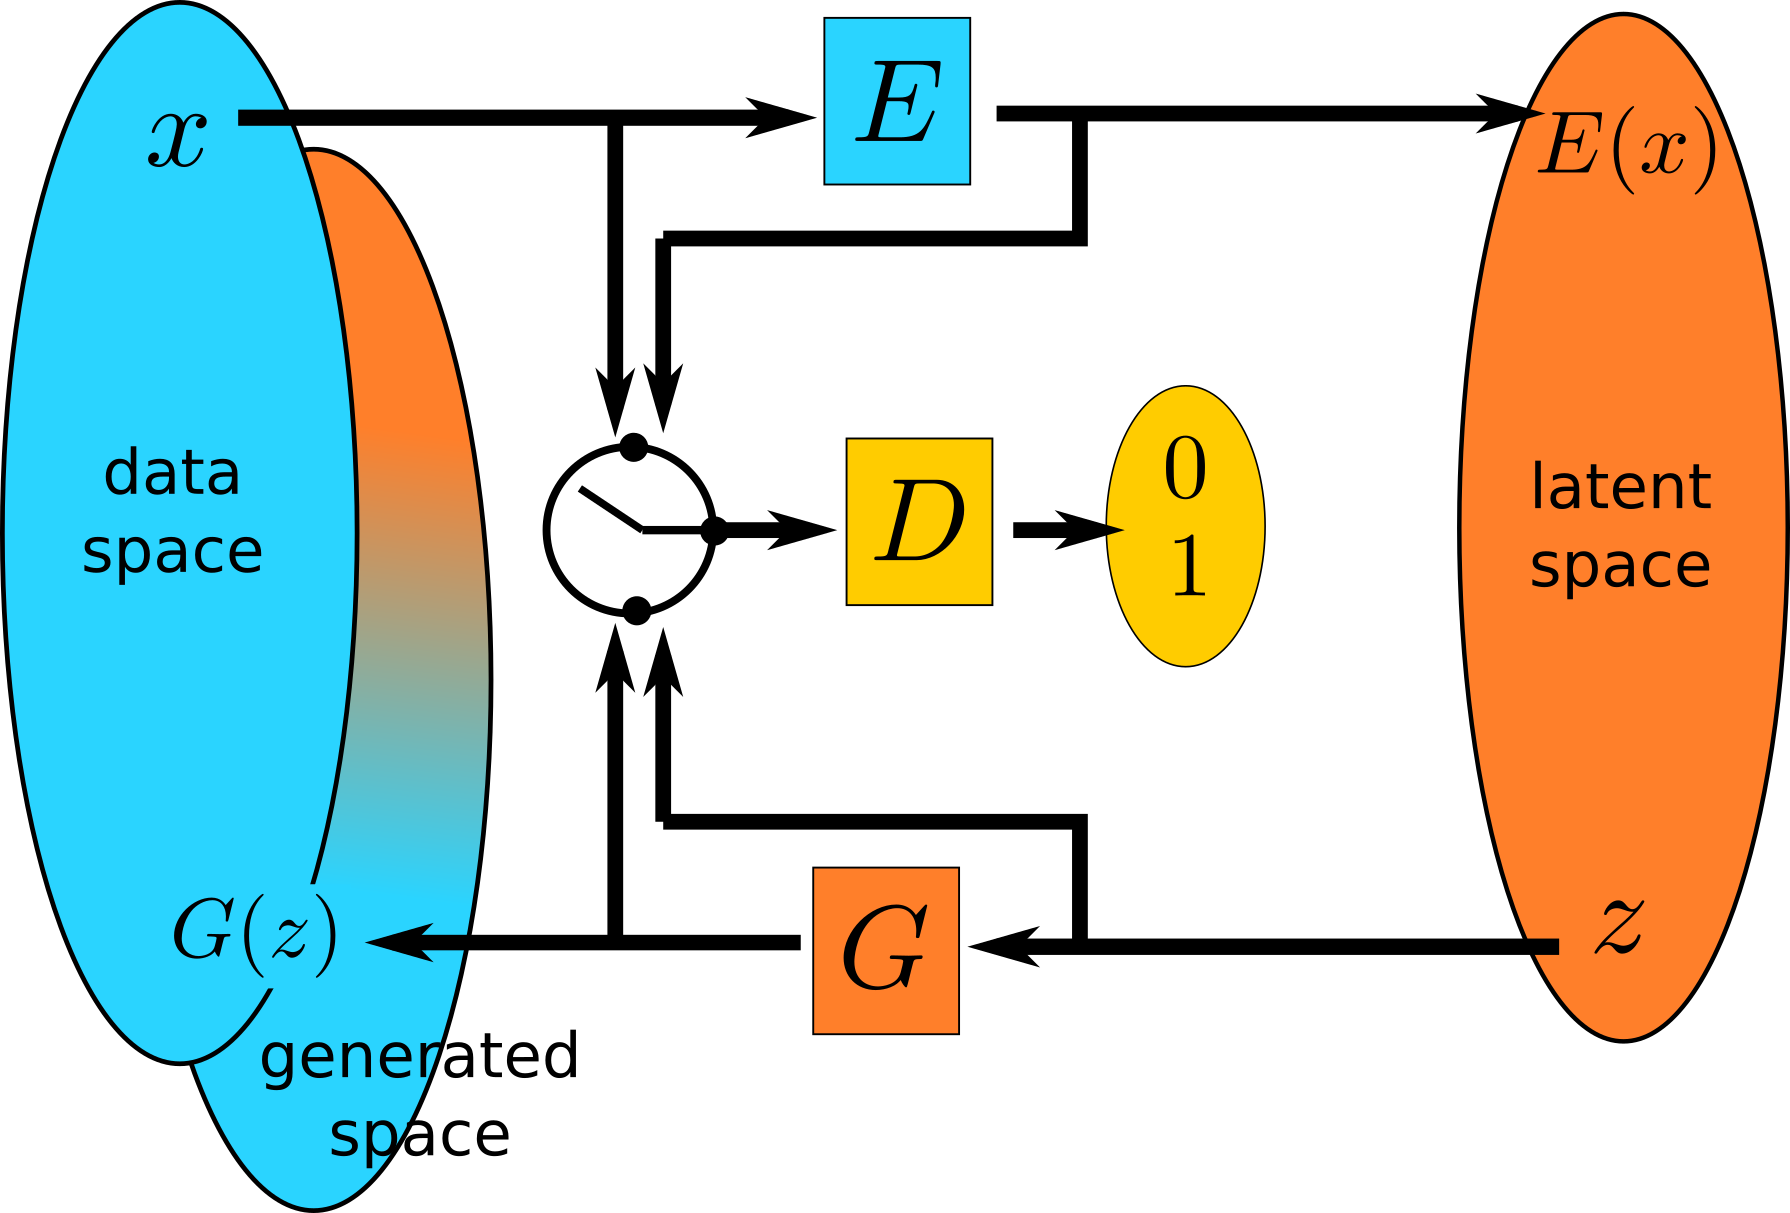
\includegraphics[width=0.6\textwidth]{bigan}
  \end{figure}

  \begin{itemize}
  \item Similar to AnoGAN, except that looking for a convenient $z^*$ for a given real image $\x$ is done using the encoder $E$
  \item Better anomaly detection results on MNIST
  \item Much faster (800x)
  \end{itemize}


\end{frame}



%%%%%%%%%%%%%%%%%%%%%%%%%%%%%%%%%%%%
\begin{frame}{GANomaly \cite{akcay_ganomaly:_2019}}

  \begin{figure}[ht]
    \centering
    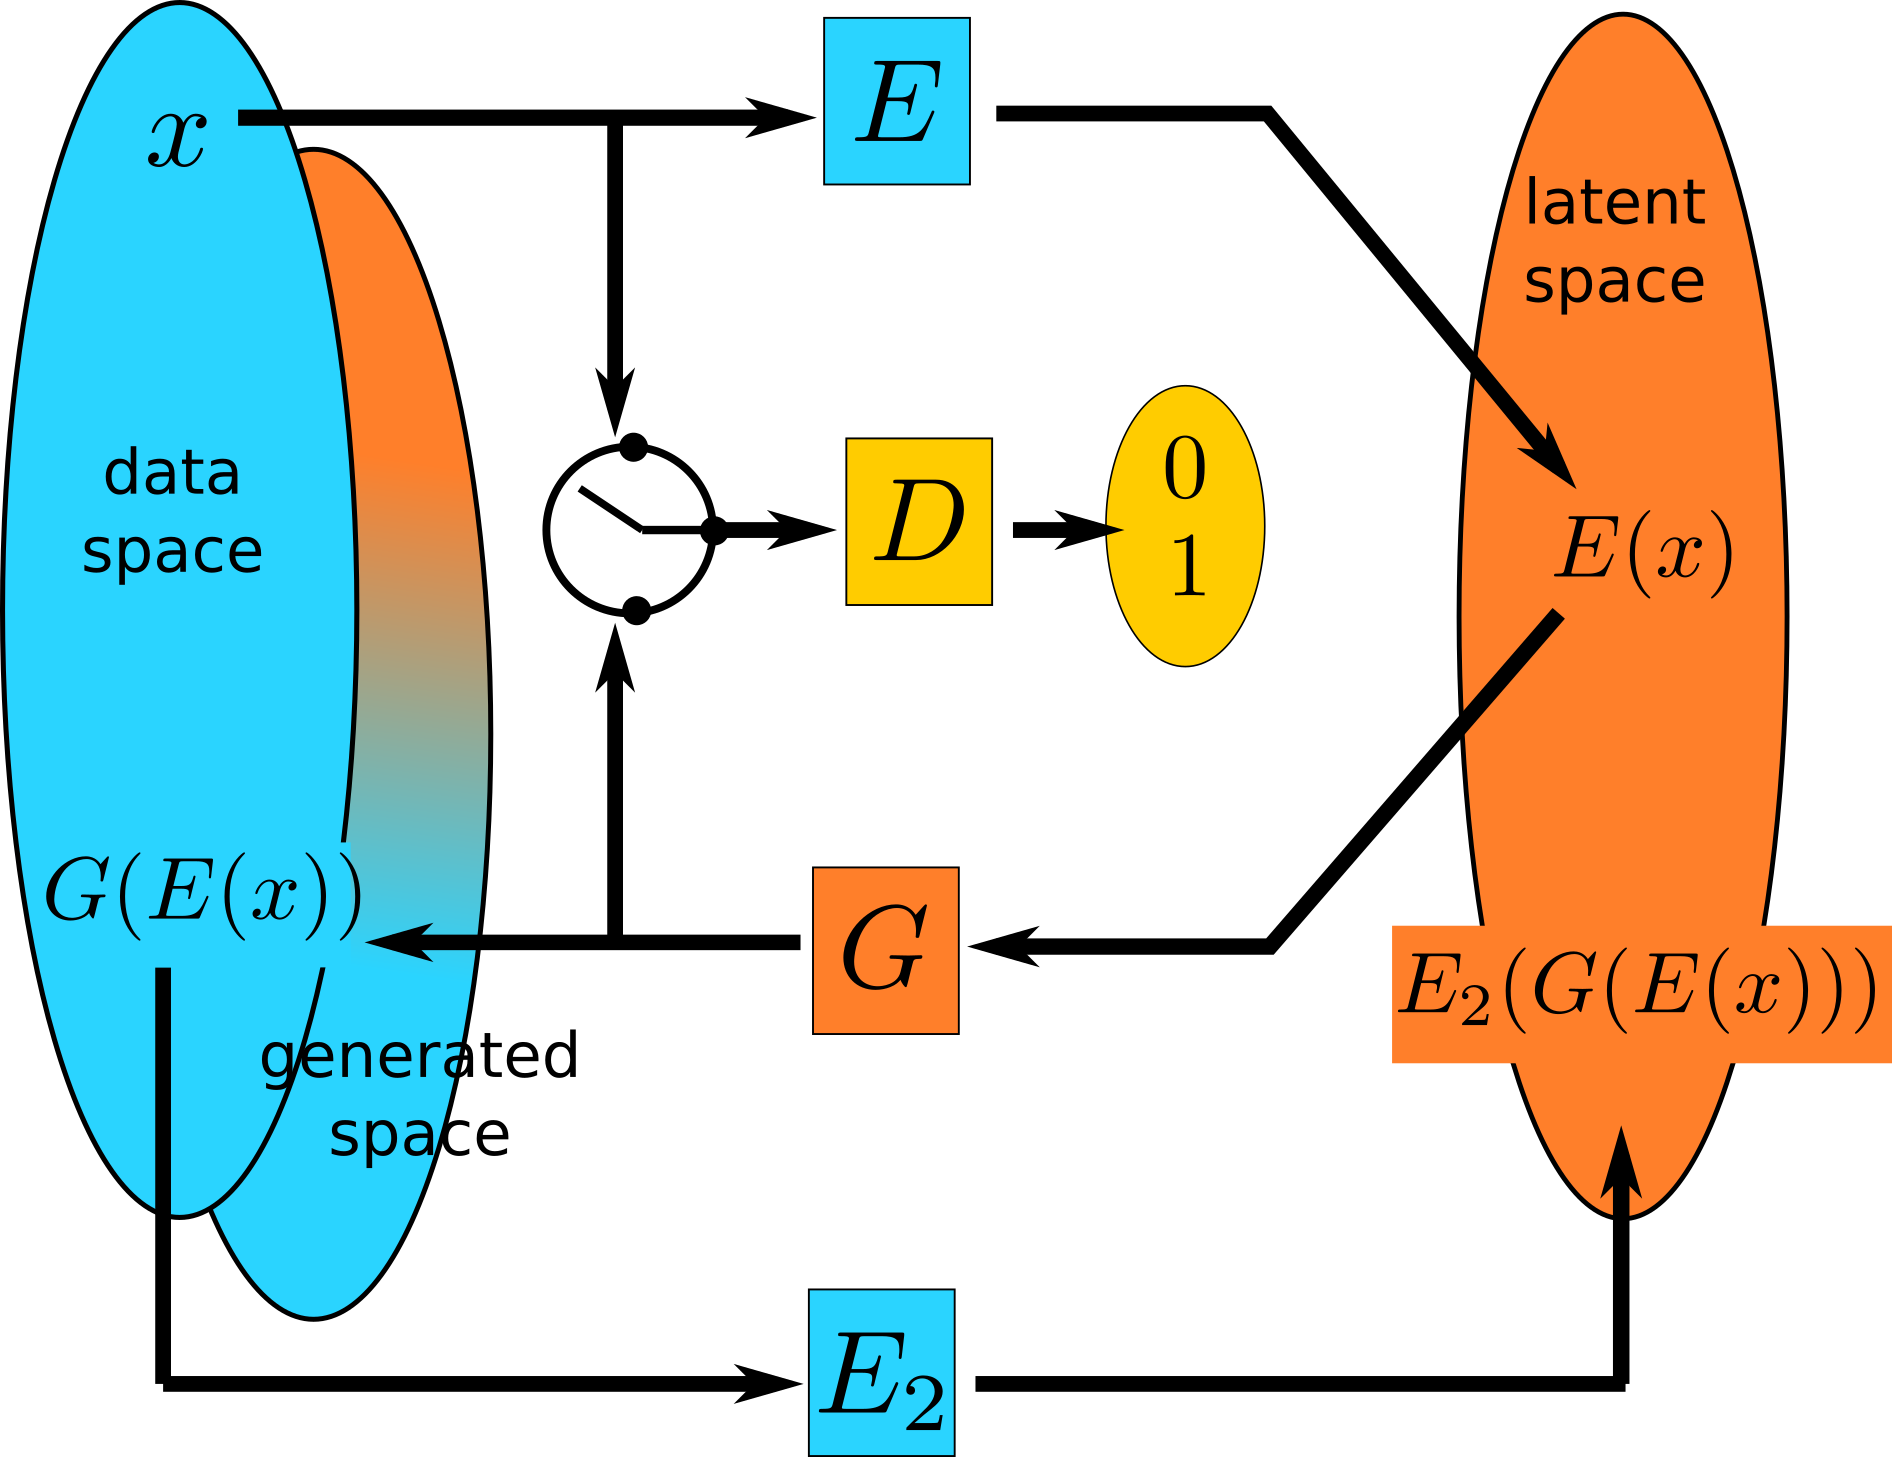
\includegraphics[width=0.6\textwidth]{ganomaly}
  \end{figure}



\end{frame}

%%%%%%%%%%%%%%%%%%%%%%%%%%%%%%%%%%%%
\begin{frame}{GANomaly : loss function}

  \begin{figure}[ht]
    \centering
    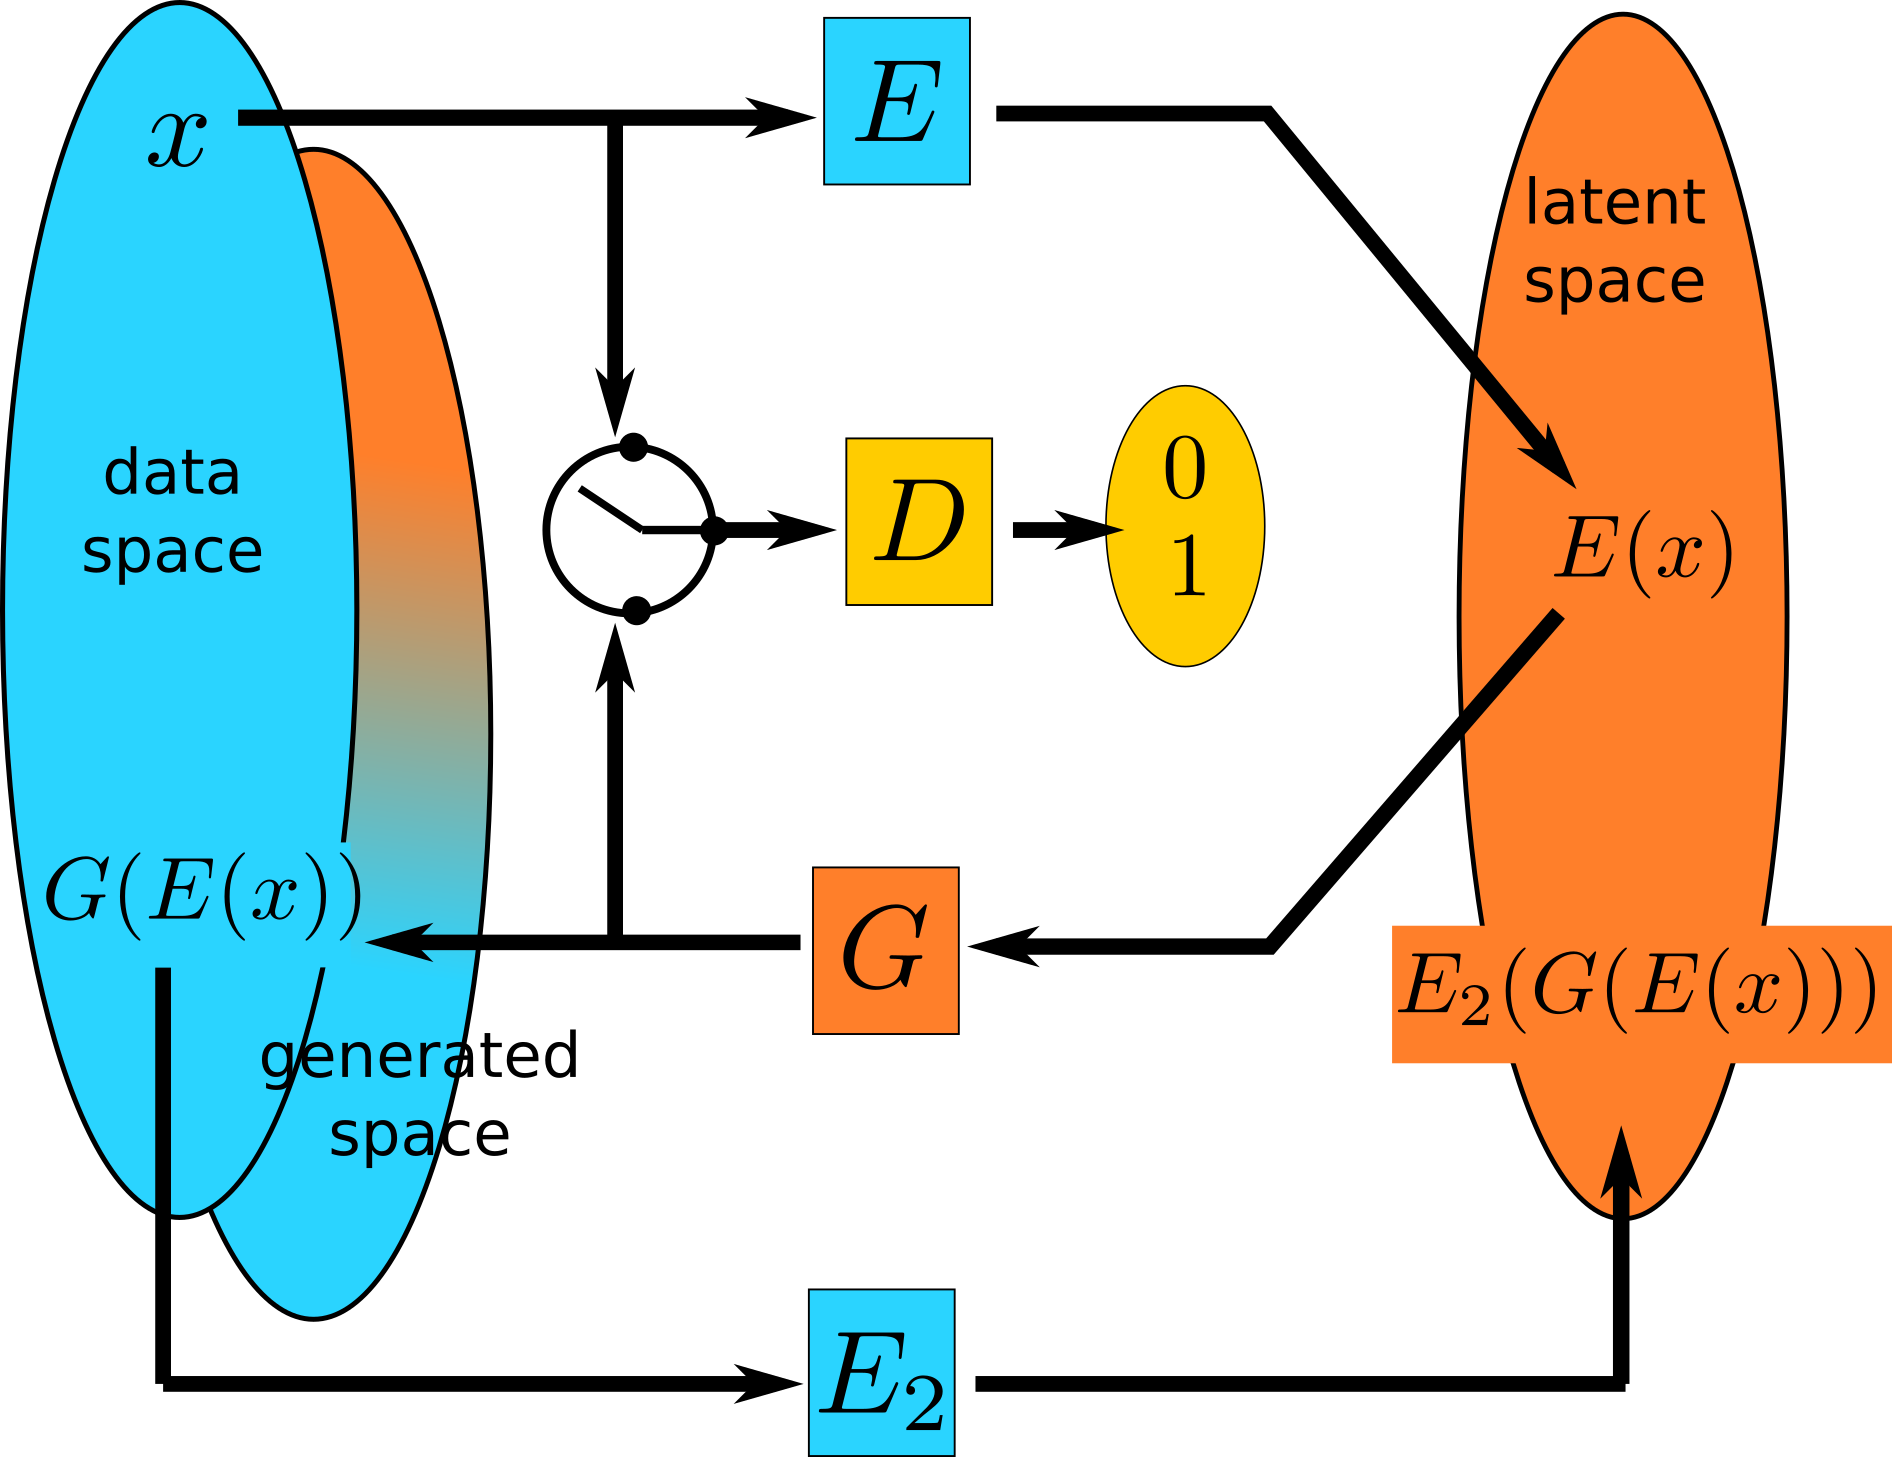
\includegraphics[width=0.4\textwidth]{ganomaly}
  \end{figure}

\small

  \begin{block}{Reconstruction loss}
    \[ \mathcal{L}_{rec}(\x) = \norm{\x - G(E(\x))}_{L_1} \]
  \end{block}

  \begin{block}{Adversarial loss}
    \[ \mathcal{L}_{adv}(\x) = \norm{f_D(\x) - f_D(G(E(\x)))}_{L_2} \]
  \end{block}

  \begin{block}{Encoding loss}
    \[ \mathcal{L}_{enc}(\x) = \norm{E(\x) - E_2(G(E(\x)))}_{L_2} \]
  \end{block}

\end{frame}


%%%%%%%%%%%%%%%%%%%%%%%%%%%%%%%%%%%%
\begin{frame}{Final loss and anomaly estimation}

  \begin{block}{Final loss}
  \[\mathcal{L} = w_{rec}\mathcal{L}_{rec} + w_{adv}\mathcal{L}_{adv} + w_{enc}\mathcal{L}_{enc}\]
  \end{block}

  \begin{block}{Anomaly estimation}
    \[A(\x) = \mathcal{L}_{enc}(\x) = \norm{E(\x) - E_2(G(E(\x)))}_{L_2} \]
  \end{block}
\end{frame}




%%%%%%%%%%%%%%%%%%%%%%%%%%%%%%%%%%%%
\begin{frame}{Comparison on MNIST}

\begin{figure}[ht]
  \centering
  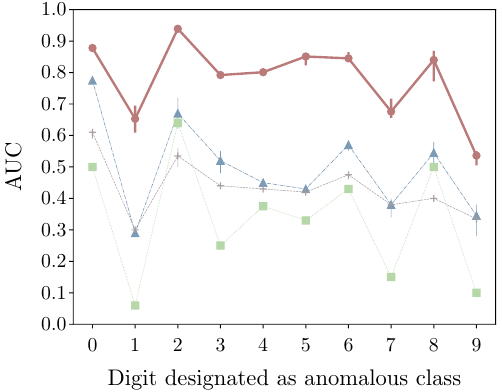
\includegraphics[width=0.8\textwidth]{comparison}
  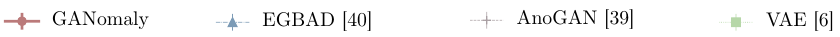
\includegraphics[width=0.8\textwidth]{comparison-legend}
  \source{\cite{akcay_ganomaly:_2019}}
\end{figure}


\end{frame}

%%%%%%%%%%%%%%%%%%%%%%%%%%%%%%%%%%%%
%%%%%%%%%%%%%%%%%%%%%%%%%%%%%%%%%%%%
\section{Using pre-trained representations}


%%%%%%%%%%%%%%%%%%%%%%%%%%%%%%%%%%%%
\begin{frame}{Getting rid of the decoder}

\end{frame}


%%%%%%%%%%%%%%%%%%%%%%%%%%%%%%%%%%%%
%%%%%%%%%%%%%%%%%%%%%%%%%%%%%%%%%%%%
\section{Conclusion}

%%%%%%%%%%%%%%%%%%%%%%%%%%%%%%%%%%%%
\begin{frame}{Conclusion}

\begin{itemize}
\item Deep learning opens new possibilities to anomalous image detection
\item Current methods need however to be improved to deal with real-world applications
\end{itemize}

\end{frame}


%%%%%%%%%%%%%%%%%%%%%%%%%%%%%%%%%%%%
\begin{frame}{Novelty generation?}

  \begin{block}{Latent space sampling~\cite{cherti_out--class_2017}}
    Sample the latent space far away from normal representations
    \begin{itemize}
    \item Will the images be realistic?
    \item Will they cover the complete range of anomalous images?
    \end{itemize}
  \end{block}

\begin{itemize}
\item See also: ``The Rules of Brainstorming Change When Artificial Intelligence Gets Involved'' (\url{https://www.ideo.com})
\end{itemize}

\end{frame}



%%%%%%%%%%%%%%%%%%%%%%%%%%%%%%%%%%%%%%%%%%%%%%%%%%
\section*{References}

%%%%%%%%%%%%%%%%%%%%%%%%%%%%%%%%%%%%%%%%%%%%%%%%%%

\frame[allowframebreaks]{

  \scriptsize

  \frametitle{References}

  %\bibliographystyle{amsalpha}
  %\bibliographystyle{apalike}

  \bibliography{../../edf.bib}

  \normalsize

}




\end{document}
